\documentclass[conference]{IEEEtran}
\IEEEoverridecommandlockouts
% TC-MIL: Topic-Chunk Multiple-Instance Learning for text-only DAIC-WOZ
% depression detection. Single-model headline + zero-shot E-DAIC transfer.
% Encoder fine-tuning extracted to sec_finetuning.tex and out of scope for
% this draft.

\usepackage{cite}
\usepackage{amsmath,amssymb,amsfonts}
\usepackage{algorithmic}
\usepackage{graphicx}
\usepackage{textcomp}
\usepackage{xcolor}
\usepackage{booktabs}
\usepackage{multirow}
\usepackage{array}
\usepackage{url}
\usepackage{tikz}
\usetikzlibrary{arrows.meta,positioning,fit,backgrounds,calc}
\usepackage{pgfplots}
\pgfplotsset{compat=1.16}
\usepackage{stfloats}            % allow table* at column bottom / better placement
% relax float limits so large tables place in-body (not after references)
\setcounter{totalnumber}{8}
\setcounter{topnumber}{4}
\setcounter{dbltopnumber}{4}
\renewcommand{\topfraction}{0.95}
\renewcommand{\bottomfraction}{0.95}
\renewcommand{\textfraction}{0.05}
\renewcommand{\floatpagefraction}{0.6}
\renewcommand{\dbltopfraction}{0.95}
\renewcommand{\dblfloatpagefraction}{0.6}
\usepackage[hidelinks]{hyperref}  % clickable cross-references (load last)
\usepackage{cleveref}
\crefname{figure}{Fig.}{Figs.}
\Crefname{figure}{Fig.}{Figs.}
\crefname{table}{Table}{Tables}
\crefname{section}{Section}{Sections}
% stacked table cell: value (+/-std) over [CI]
\newcommand{\celld}[3]{\shortstack{#1{\footnotesize\,$\pm$#2}\\[-1.5pt]{\tiny[#3]}}}
\def\BibTeX{{\rm B\kern-.05em{\sc i\kern-.025em b}\kern-.08em
    T\kern-.1667em\lower.7ex\hbox{E}\kern-.125emX}}

\begin{document}

\title{Topic-Chunk Multiple-Instance Learning for\\Text-Only Depression
Detection on DAIC-WOZ\\Under a Leakage-Free Evaluation Protocol}

\author{\IEEEauthorblockN{Saverio Napolitano}
\IEEEauthorblockA{\textit{Dept. of Engineering Enzo Ferrari} \\
\textit{University of Modena and Reggio Emilia}\\
Modena, Italy \\
302341@studenti.unimore.it} % substitute with ORCID
\and
\IEEEauthorblockN{Biagio Carpaneto}
\IEEEauthorblockA{\textit{Dept. of Engineering Enzo Ferrari} \\
\textit{University of Modena and Reggio Emilia}\\
Modena, Italy \\
276275@studenti.unimore.it} % substitute with ORCID
}

\maketitle

\begin{abstract}
Automatic depression detection from clinical-interview transcripts is
attractive, but progress on the DAIC-WOZ benchmark is obscured by two problems:
a representation bottleneck when each instance is a single conversational turn,
and evaluation protocols that are not comparable across papers and can
leak information through pooled cross-validation, test-tuned thresholds, or the
interviewer-prompt shortcut. We present TC-MIL, a topic-chunk Multiple-Instance
Learning model that treats short sliding windows of dialogue as instances,
embeds them with a frozen sentence encoder, aggregates them with gated-attention
pooling over a recurrent context, and is regularised by an auxiliary PHQ-8
symptom head. Evaluated strictly on the official AVEC2017 split (per-seed mean
over 30 seeds, an a-priori prevalence threshold, a single test evaluation), a
single TC-MIL network reaches macro-F1 0.774, micro-F1 0.814 and ROC-AUC 0.864,
significantly exceeding the cleanest validity-checked text-only baseline and
matching the strongest reported text-only single model within seed variation. Ablations localise the gain in the dialogue-chunk
representation and in removing a recall-biasing class weight, cross-validation
corroborates the ranking, and interpretability analysis shows the attention is
cross-seed stable, free of the prompt shortcut, and clinically grounded, while
not a faithful per-instance explanation.
\end{abstract}

\begin{IEEEkeywords}
depression detection, multiple-instance learning, DAIC-WOZ, clinical NLP,
attention, interpretability, evaluation protocol
\end{IEEEkeywords}

\section{Introduction}

Major depressive disorder is among the most prevalent mental-health
conditions, and the standard screening instrument, the eight-item Patient
Health Questionnaire (PHQ-8), is administered through structured questions
about sleep, mood, energy, appetite and related constructs. The DAIC-WOZ
corpus \cite{gratch2014,devault2014} pairs transcripts of semi-structured
clinical interviews with PHQ-8 scores, and has become the principal public
benchmark for automatic depression detection. Among its modalities, \emph{text} is the most portable: it requires
no acoustic or visual capture, is straightforward to de-identify, and isolates
the linguistic content of what a participant says.

Despite a large literature, the text-only DAIC-WOZ task suffers from two
problems that make reported numbers hard to trust and harder to compare.

\textbf{A representation bottleneck.} Most prior systems treat each
participant turn as the unit of classification or of Multiple-Instance
Learning (MIL). The majority of DAIC-WOZ turns are short backchannels
(``yeah'', ``mhm'', ``i don't know''); a frozen sentence encoder maps these to
near-identical vectors, so no pooling mechanism, however elaborate, can recover
a signal the instances do not carry. We observed this ceiling directly across
thirty-five iterations of a role-aware utterance-MIL family that plateaued at
positive-class F1 between 0.50 and 0.58 regardless of how many regularisers
(focal loss, label smoothing, manifold mixup, stochastic weight averaging,
gradient normalisation, adversarial perturbation) were stacked on top.

\textbf{An evaluation-protocol problem.} Published DAIC-WOZ numbers are
reported on different splits (dev vs.\ official test vs.\ pooled
cross-validation), with different F1 variants (positive-class vs.\ macro
vs.\ micro), and frequently with information leakage: thresholds tuned on test
labels, probability ensembles over folds that share subjects, or reliance on
the interviewer-prompt shortcut that Burdisso et al.\ \cite{burdisso2024}
showed can be exploited to reach macro-F1 0.90 by feeding the model the
therapist's mental-health questions. A method that is not measured under a
fixed, leakage-free protocol cannot be compared on equal terms with the literature.

\textbf{Contributions.} This paper makes three contributions.
\begin{enumerate}
\item \textbf{TC-MIL}, a topic-chunk MIL model whose instances are short
sliding windows of dialogue rather than single turns. The chunk restores the
topical context (a question about sleep and the answer to it) that PHQ-8
symptoms attach to, turning near-degenerate instances into discriminative
ones (\Cref{sec:method}).
\item A \textbf{leakage-free evaluation protocol} on the official AVEC2017
split --- per-seed mean$\pm$std over 30 seeds, a-priori prevalence thresholds, a
single test evaluation, and non-parametric and parametric significance testing
--- under which a single TC-MIL network beats the cleanest validity-checked
text-only baseline on positive-, macro- and micro-F1 and on AUC, and matches the
strongest reported text-only single model within seed variation
(\Cref{sec:protocol,sec:external}).
\item \textbf{Extensive validation} under that protocol: an architecture
ablation and single-lever study that localise the gain in the chunk
representation and the removal of a recall-biasing class weight, an internal
cross-validation that corroborates the ranking, and a quantified
interpretability analysis of attention faithfulness, the clinical symptom
read-out, and the interviewer-prompt bias probes
(\Cref{sec:ablation,sec:internal,sec:interpret}).
\end{enumerate}

\section{Related Work and Baseline Selection}
\label{sec:related}

A central difficulty in positioning a DAIC-WOZ result is that many headline
numbers are not directly comparable: they are measured on the development set, on a
non-standard split, on a different modality, or with the interviewer-prompt
shortcut left uncontrolled. We therefore organise this section around a validity
filter, comparing primarily against results that are on the held-out test set,
text-only, and outside the interviewer-prompt-inflated regime identified by
\cite{burdisso2024}.

\textbf{The validity filter.} \cite{burdisso2024} demonstrate
that including the interviewer's (``Ellie'') prompts inflates DAIC-WOZ scores
through a positional shortcut: a model reading only the second half of the
interview, where explicit mental-health questions are asked, scores far higher.
Their clean patient-only model reaches macro-F1 0.85, an Ellie-prompt model
0.88, and a deliberately bias-exploiting combination 0.90. The lesson is
methodological, not a magnitude cut-off: a baseline falls outside the clean
regime if it feeds the model interviewer prompts or the late question region
without controlling for the shortcut, which drives scores into the 0.88--0.90 band.

\textbf{Primary baseline.} Milintsevich et al.\ \cite{milintsevich2023}
predict the eight PHQ-8 symptom severities with a hierarchical regressor
(sentence-RoBERTa turn encoder, BiLSTM interview encoder with additive
attention) and threshold for the binary task. It is the cleanest comparable
baseline because it (a) reports on the held-out test split, (b) contains an
in-paper validity check --- perturbing the participants' yes/no answers caused
no micro-F1 drop and only a 0.52\% macro-F1 drop, and saliency attends symptom
turns rather than the diagnosis question --- and (c) its macro-F1 of 0.739
sits well inside the clean regime. It reports both micro-F1 (0.766) and
macro-F1 (0.739); we match both.

\textbf{Other test-set numbers.} To the best of our knowledge, only a few papers
in the literature are both test-set and text-only single models. Beyond
\cite{milintsevich2023}, these are the multi-view models of Agarwal et al.\
(macro-F1 0.732 \cite{agarwal2022mv}, 0.80 \cite{agarwal2024}), HCAN
\cite{mallolragolta2019} (positive-class F1 0.63), the affective HAN of
\cite{xezonaki20_interspeech} (macro-F1 0.70), and the Bi-LSTM with self-attention
of \cite{10006532} (macro-F1 0.78 with interviewer prompts, 0.72 participant-only).
This paper therefore leads the cleanest
\emph{verified single-model} test-set baseline \cite{milintsevich2023} and matches
the best reported text-only single model within seed variation
(\Cref{sec:external}).

\section{Method: TC-MIL}
\label{sec:method}

TC-MIL classifies an interview as a bag of instances under the standard MIL
assumption that a bag is positive if it contains evidence of depression. Its
design is intentionally minimal: the discriminative power comes from the
instance definition rather than from a heavy aggregation network.
\Cref{fig:arch} shows the full pipeline.

\begin{figure*}[t]
\centering
\resizebox{\textwidth}{!}{%
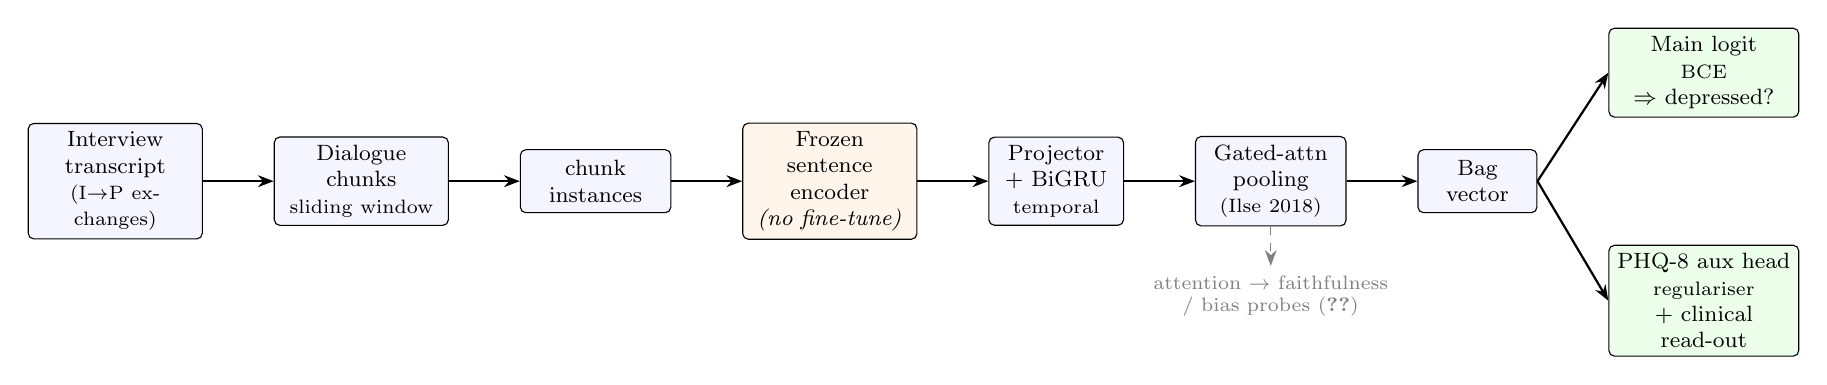
\begin{tikzpicture}[
  node distance=6mm and 9mm,
  font=\footnotesize,
  box/.style={draw, rounded corners=2pt, align=center, minimum height=8mm,
              inner sep=3pt, fill=blue!4},
  enc/.style={box, fill=orange!8},
  head/.style={box, fill=green!8},
  freeze/.style={box, fill=gray!10},
  >={Stealth[length=2mm]},
  arr/.style={->, thick},
]
% --- input ---
\node[box, text width=20mm] (interview)
  {Interview\\transcript\\{\scriptsize (I$\rightarrow$P exchanges)}};
\node[box, right=of interview, text width=20mm] (chunk)
  {Dialogue\\chunks\\{\scriptsize sliding window}};
% stacked instances cue
\node[box, right=of chunk, text width=17mm, fill=blue!4] (inst)
  {chunk\\instances};
\node[box, right=of inst, enc, text width=20mm] (encoder)
  {Frozen sentence\\encoder\\\textit{(no fine-tune)}};
\node[box, right=of encoder, text width=15mm] (proj)
  {Projector\\$+$ BiGRU\\{\scriptsize temporal}};
\node[box, right=of proj, text width=17mm] (attn)
  {Gated-attn\\pooling\\{\scriptsize (Ilse 2018)}};
\node[box, right=of attn, text width=13mm] (bag)
  {Bag\\vector};
% --- heads ---
\node[head, above right=4mm and 9mm of bag, text width=22mm] (main)
  {Main logit\\{\scriptsize BCE}\\$\Rightarrow$ depressed?};
\node[head, below right=4mm and 9mm of bag, text width=22mm] (aux)
  {PHQ-8 aux head\\{\scriptsize regulariser}\\$+$ clinical read-out};
% --- arrows ---
\draw[arr] (interview) -- (chunk);
\draw[arr] (chunk) -- (inst);
\draw[arr] (inst) -- (encoder);
\draw[arr] (encoder) -- (proj);
\draw[arr] (proj) -- (attn);
\draw[arr] (attn) -- (bag);
\draw[arr] (bag.east) -- (main.west);
\draw[arr] (bag.east) -- (aux.west);
% attention weights feed interpretability (dashed back-annotation)
\node[below=5mm of attn, gray, font=\scriptsize, align=center] (interp)
  {attention $\to$ faithfulness\\/ bias probes (\Cref{sec:interpret})};
\draw[->, dashed, gray] (attn.south) -- (interp.north);
\end{tikzpicture}}
\caption{TC-MIL pipeline. An interview is split into overlapping dialogue
chunks; each chunk is embedded by a
\emph{frozen} sentence encoder, contextualised by a residual BiGRU, and
aggregated by gated-attention pooling into one bag vector. A main logit (BCE) gives the depression decision; an auxiliary PHQ-8
symptom head regularises the backbone and doubles as the clinical read-out.
The attention weights are the surface analysed for faithfulness and
interviewer-prompt bias in \Cref{sec:interpret}.}
\label{fig:arch}
\end{figure*}

\subsection{Dialogue-chunk instances}
Let an interview be a sequence of (interviewer$\rightarrow$participant)
exchanges. We form instances with a sliding window of $w$ consecutive
exchanges and stride $s$, rendering each window as plain dialogue text. With
$w=4,\ s=2$ this yields on the order of 28 instances per interview, each
$\approx$65 words, so a window contains a question and its answer ---
``how have you been sleeping?'' together with the response --- restoring the
context that a single backchanneled turn lacks (\Cref{fig:chunk}). Our
development ablations indicate this is the most influential design choice:
widening the window from 2 to 4--6 exchanges is what separates an effective model
from an ineffective one.

\begin{figure}[t]
\centering
\resizebox{\columnwidth}{!}{%
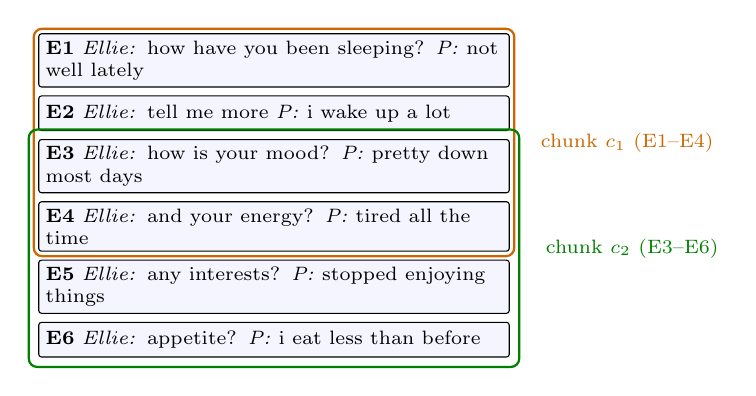
\begin{tikzpicture}[
  font=\scriptsize,
  ex/.style={draw, rounded corners=1pt, text width=58mm, align=left,
             inner sep=2.5pt, fill=blue!4, minimum height=4.4mm},
  >={Stealth[length=1.6mm]},
]
\node[ex] (e1) {\textbf{E1} \emph{Ellie:} how have you been sleeping? \emph{P:} not well lately};
\node[ex, below=1.0mm of e1] (e2) {\textbf{E2} \emph{Ellie:} tell me more \emph{P:} i wake up a lot};
\node[ex, below=1.0mm of e2] (e3) {\textbf{E3} \emph{Ellie:} how is your mood? \emph{P:} pretty down most days};
\node[ex, below=1.0mm of e3] (e4) {\textbf{E4} \emph{Ellie:} and your energy? \emph{P:} tired all the time};
\node[ex, below=1.0mm of e4] (e5) {\textbf{E5} \emph{Ellie:} any interests? \emph{P:} stopped enjoying things};
\node[ex, below=1.0mm of e5] (e6) {\textbf{E6} \emph{Ellie:} appetite? \emph{P:} i eat less than before};
% windows (w=4, s=2)
\node[draw=orange!80!black, thick, rounded corners=3pt,
      fit=(e1)(e4), inner sep=1.6pt] (w1) {};
\node[draw=green!50!black, thick, rounded corners=3pt,
      fit=(e3)(e6), inner sep=3.4pt] (w2) {};
\node[orange!80!black, anchor=west] at ([xshift=2mm]w1.east) {chunk $c_1$ (E1--E4)};
\node[green!50!black, anchor=west] at ([xshift=2mm]w2.east) {chunk $c_2$ (E3--E6)};
\end{tikzpicture}}
\caption{Dialogue-chunk instances (illustrative). A sliding window of $w{=}4$
exchanges with stride $s{=}2$ turns the interview into overlapping chunks: $c_1$
spans exchanges E1--E4, $c_2$ spans E3--E6, and so on. Each chunk is rendered as
one plain-text passage of several question--answer pairs (here sleep, mood,
energy), so a single instance already carries the topical context that an
isolated turn lacks. Text is synthetic, not from DAIC-WOZ.}
\label{fig:chunk}
\end{figure}

\subsection{Frozen sentence encoder}
Each chunk is embedded with a frozen sentence encoder
(\texttt{bge-large-en-v1.5}, 335M parameters, 1024-dimensional mean-pooled
output). Freezing the encoder is a deliberate choice given only 107 training
subjects: it removes the dominant overfitting risk and makes the experiments
cheap and reproducible.

\subsection{Gated-attention pooling with a temporal context}
A small projector reduces the chunk embeddings, an optional one-layer
bidirectional GRU (residual) lets each chunk see its conversational
neighbourhood, and a gated-attention pooling layer \cite{ilse2018} produces a
single bag vector as an attention-weighted sum of instances. In our ablations the
GRU is the next most influential component after chunking, adding 0.02--0.03
development AUC across encoders; a transformer context was unstable at this sample size, so
the recurrent inductive bias is preferred. The whole head is on the order of
$10^5$ parameters and uses none of the mixup, focal, SWA, or diversity losses
of the prior family.

\subsection{Auxiliary PHQ-8 symptom head}
A second head predicts the eight binarised PHQ-8 items from the pooled vector.
It shares the backbone but does \emph{not} feed the main logit; it is a pure
regulariser worth $\approx$0.02 development AUC, and it doubles as the
clinical read-out probed in \Cref{sec:interpret}.

\subsection{Loss and the positive class weight}
The main objective is a binary cross-entropy on the bag logit plus the
weighted auxiliary loss. The DAIC-WOZ training split is imbalanced
($\approx$28\% positive), and a class weight of (neg/pos)$\approx$2.5 is the
natural default --- but it biases the model toward recall. As
\Cref{sec:ablation} shows, setting this weight to 1.0 is the single
change that closes the residual F1 gap, because it produces less skewed
probabilities so that a fixed prevalence threshold lands nearer the
F1-optimal operating point.

\section{Evaluation Protocol}
\label{sec:protocol}

We describe the protocol in detail, because the limited comparability of the
existing literature is itself one of the observations that motivates this work.

\textbf{Splits.} We use the official AVEC2017 split: 107 train, 35 dev, 47
test subjects, subject-disjoint by construction. The encoder
sees training text only; the dev set is used for early stopping and threshold
estimation; the test set is evaluated \emph{once} per reported configuration.

\textbf{Thresholding.} The 35-subject dev set is too small for F1/balanced-
accuracy/Youden tuning, which all collapse to a degenerate $t\!\approx\!0.15$
with recall pinned at 1.0. We instead use an \emph{a-priori prevalence}
threshold: choose $t$ so that the predicted positive rate matches the training
prevalence ($\approx$0.28). This uses the model's scores and a training-derived
prior but never a test label, so it is leakage-free.

\textbf{Metrics.} We report ROC-AUC (threshold-free ranking), positive-class
F1, macro-F1, micro-F1 (which equals accuracy for single-label binary
classification), and the unweighted average recall (UAR --- the mean of the
per-class recalls, identical to balanced accuracy), the last being the standard
balanced metric in the depression-detection literature. Both threshold-dependent metrics are computed at the
same a-priori prevalence threshold as macro-F1, so they are honest and not
separately tuned oracles.

\textbf{Seeds and reporting.} Every
official-split number is a per-seed mean$\pm$std over 30 seeds, rather than a
single run or a seed ensemble. We additionally report a subject-level bootstrap
confidence interval to characterise the uncertainty inherent in a 47-subject
test set.

\textbf{Significance.} Two regimes are used. For the official split, the 30
per-seed metrics of two models are \emph{independent} samples, compared with
the Mann--Whitney $U$ test and Welch's $t$-test. For cross-validation, the
fold-and-seed-matched metrics are \emph{paired} (identical fold membership via
a shared split seed), compared with the Wilcoxon signed-rank test and the
paired $t$-test. Against the external baseline, whose per-subject scores are
not public, we use a one-sample $t$-test of our 30 per-seed macro-F1 values
against the reported 0.739.

\section{External Comparison Against the Literature}
\label{sec:external}

\Cref{tab:external} is the headline result: a single TC-MIL network on the
official test split against the verified leakage-free text-only single-model
baselines. For direct comparison the table shows only the metrics the text-only
literature reports; the full metric set for TC-MIL and the internal baselines is
in \Cref{tab:ladder}. The TC-MIL cells are the 30-seed per-seed mean$\pm$std at
the a-priori prevalence threshold, where pos-F1 is the positive-class F1 and
macro-F1 the both-class mean.

\begin{table}[t]
\caption{Official AVEC2017 test split against the verified leakage-free
text-only single-model literature. TC-MIL cells are the 30-seed
per-seed mean$\,{\pm}\,$std (top) and the subject-level bootstrap 95\% CI
(bottom, 2000 resamples of the 47 test subjects). ``--'' $=$ not
reported.}
\label{tab:external}
\centering
\small
\setlength{\tabcolsep}{4pt}
\resizebox{\columnwidth}{!}{%
\begin{tabular}{@{}lccccc@{}}
\toprule
\textbf{Method} & \textbf{pos-F1} & \textbf{micro-F1} & \textbf{macro-F1} & \textbf{UAR} & \textbf{ROC-AUC} \\
\midrule
HCAN \cite{mallolragolta2019} (2019) & 0.63 & -- & -- & 0.66 & -- \\
HAN+L \cite{xezonaki20_interspeech} (2020) & -- & -- & 0.70 & 0.70 & -- \\
Bi-LSTM+Attn \cite{10006532} (2022) & -- & -- & 0.7834 & 0.7857 & -- \\
Agarwal MV-IA \cite{agarwal2022mv} (2022) & -- & 0.7173 & 0.7319 & 0.7232 & -- \\
Milintsevich \cite{milintsevich2023} (2023) & -- & 0.766{\footnotesize$\pm$.023} & 0.739{\footnotesize$\pm$.025} & -- & -- \\
Agarwal multi-view \cite{agarwal2024} (2024) & -- & -- & 0.80 & 0.83 & -- \\
\addlinespace[2pt]
\textbf{TC-MIL (ours)} & \celld{\textbf{.68}}{.04}{.41,.86} & \celld{\textbf{.81}}{.02}{.66,.92} & \celld{\textbf{.77}}{.03}{.59,.90} & \celld{\textbf{.77}}{.03}{.59,.92} & \celld{\textbf{.86}}{.01}{.75,.96} \\
\bottomrule
\end{tabular}}
\end{table}

The single TC-MIL network significantly exceeds \cite{milintsevich2023} on the
metrics that work reports: micro-F1 0.814 vs.\ 0.766 and macro-F1 0.774 vs.\
0.739 (one-sample $t$ over 30 seeds, $p=3.8\!\times\!10^{-7}$), and it adds a
threshold-free AUC of 0.864 that the baseline does not report.

Two single-run results report a higher macro-F1. The strongest prior text-only
single model is the multi-view network of \cite{agarwal2024}, which reports a
single-run test macro-F1 of 0.80 on the same split; our 30-seed mean
$0.774\pm0.029$ places that value within about one standard deviation, so on
macro-F1 the two are statistically indistinguishable under seed variation. The
Bi-LSTM with self-attention of \cite{10006532} reports $0.7834$, but that is its
dialogue setting that ingests the interviewer's questions --- the prompt shortcut
we control for (\Cref{sec:interpret}) --- and its participant-only setting falls to
$0.7235$; it too sits within one seed standard deviation of $0.774\pm0.029$. Both
are single runs without an AUC, a micro-F1, an interviewer-prompt bias control, or
a subject-level interval.

On UAR (\Cref{tab:external}) the picture is consistent: our $0.77\pm0.03$ exceeds
\cite{mallolragolta2019} ($0.66$), \cite{xezonaki20_interspeech} ($0.70$) and
\cite{agarwal2022mv} ($0.7232$), and sits within one seed standard deviation of
the Bi-LSTM ($0.7857$, unchanged across its dialogue and participant-only
settings); \cite{agarwal2024} reports a higher single-run UAR of $0.83$, but that
point falls inside our subject-level bootstrap interval $[0.59, 0.92]$, so on 47
test subjects the difference is not resolvable.

In sum, TC-MIL matches the best prior text-only single model on macro-F1 and is
competitive on UAR. Beyond the point estimates it supplies a threshold-free AUC
(0.864), micro-F1 (0.814), an explicit bias control, a per-chunk faithfulness
analysis, and 30-seed plus bootstrap uncertainty. The subject-level bootstrap
intervals for the headline operating point are wide (ROC-AUC $[0.751, 0.963]$,
macro-F1 $[0.591, 0.898]$ over 2000 resamples of the 47 test subjects,
\Cref{tab:external}); every DAIC-WOZ test number carries this uncertainty, and we
report it as an integral part of the protocol.

\section{Finding the Best Model: Ablations}
\label{sec:ablation}

Two ablations, both under the protocol of \Cref{sec:protocol}, explain
\emph{why} TC-MIL works: an architecture ladder that isolates the contribution
of the chunk representation, and a single-lever study that isolates the final
F1 improvement.

\subsection{Architecture ladder}
\Cref{tab:ladder} re-trains the full lineage --- a context-free dialogue
mean, flat utterance-MIL with mean and with gated-attention pooling, the
role-aware DAMIL-R, the symptom-supervised SS-DAMIL-R variants, and TC-MIL ---
from scratch on the full dataset under the identical 30-seed single-model
protocol.

The two role-aware families are our own prior baselines on this task. \textbf{DAMIL-R} (\emph{Dual-Attention MIL, Role-aware}) keeps the
utterance as the instance but adds a dual cross-role attention: it pools the
participant turns and the interviewer turns through separate attention streams
and lets each condition on the other, so that an answer is read in the light of
the question that prompted it. This rebuilds part of the dialogue context that
a flat utterance bag discards, and it is the single largest jump in the legacy
ladder (\Cref{tab:ladder}). \textbf{SS-DAMIL-R} (\emph{Symptom-Supervised
DAMIL-R}) adds a PHQ-8 symptom-prediction objective on top of DAMIL-R --- the
same idea TC-MIL later reuses as a pure auxiliary regulariser. \emph{SS-DAMIL-R\,(MH)} is the canonical symptom-supervised model with \emph{multi-head}
pooling and is the legacy ceiling; \emph{SS-DAMIL-R\,(GSI)} replaces the
additive symptom signal with a \emph{gated symptom-injection} block; and
\emph{SS-DAMIL-R\,(Conv)} prepends a 1-D \emph{convolutional} front-end
over the participant sequence before the cross-role attention. The
remaining experiments in this family are augmentation-hyper\-
parameter permutations of the MH architecture (mixup, instance/word dropout,
auxiliary-loss schedules, test-time augmentation) and collapse onto it under
the leakage-free protocol, which is why only the three distinct classes appear
here.

\begin{table*}[t]
\caption{Architecture ladder, official split, full metric set at the a-priori
prevalence threshold. Each cell is the 30-seed per-seed mean$\,{\pm}\,$std
(top) and the subject-level bootstrap 95\% CI (bottom, 2000 resamples of the
47 test subjects). Instances are single utterances except for TC-MIL
(dialogue chunks).}
\label{tab:ladder}
\centering
\scriptsize
\setlength{\tabcolsep}{3pt}
\begin{tabular}{@{}lcccccccc@{}}
\toprule
\textbf{Architecture} & \textbf{UAR} & \textbf{Prec.} & \textbf{Recall} & \textbf{pos-F1} & \textbf{macro-F1} & \textbf{micro-F1} & \textbf{PR-AUC} & \textbf{ROC-AUC} \\
\midrule
dialogue mean & \celld{.56}{.06}{.45,.76} & \celld{.27}{.26}{.00,.58} & \celld{.26}{.26}{.00,.86} & \celld{.24}{.23}{.00,.67} & \celld{.51}{.10}{.38,.71} & \celld{.68}{.04}{.47,.77} & \celld{.50}{.07}{.27,.73} & \celld{.66}{.04}{.47,.82} \\
\addlinespace[2pt]
flat MIL, mean & \celld{.51}{.02}{.50,.50} & \celld{.11}{.18}{.00,.00} & \celld{.08}{.14}{.00,.00} & \celld{.09}{.14}{.00,.00} & \celld{.45}{.05}{.36,.47} & \celld{.68}{.04}{.55,.83} & \celld{.40}{.09}{.22,.63} & \celld{.61}{.08}{.42,.75} \\
\addlinespace[2pt]
flat MIL, attn & \celld{.53}{.04}{.45,.77} & \celld{.22}{.25}{.19,.73} & \celld{.18}{.20}{.18,.71} & \celld{.18}{.19}{.19,.67} & \celld{.48}{.08}{.45,.76} & \celld{.67}{.04}{.53,.81} & \celld{.48}{.10}{.31,.78} & \celld{.67}{.09}{.57,.86} \\
\addlinespace[2pt]
DAMIL-R & \celld{.66}{.06}{.53,.85} & \celld{.55}{.09}{.29,.85} & \celld{.50}{.12}{.31,.80} & \celld{.51}{.10}{.31,.77} & \celld{.66}{.06}{.53,.84} & \celld{.73}{.05}{.62,.87} & \celld{.59}{.08}{.38,.84} & \celld{.75}{.06}{.64,.90} \\
\addlinespace[2pt]
SS-DAMIL-R (MH)& \celld{.67}{.06}{.51,.85} & \celld{.58}{.11}{.29,.85} & \celld{.51}{.13}{.29,.80} & \celld{.53}{.12}{.30,.77} & \celld{.67}{.07}{.51,.84} & \celld{.74}{.03}{.60,.87} & \celld{.60}{.08}{.39,.84} & \celld{.76}{.05}{.62,.91} \\
\addlinespace[2pt]
SS-DAMIL-R (GSI)& \celld{.66}{.06}{.53,.84} & \celld{.53}{.09}{.31,.83} & \celld{.50}{.12}{.31,.80} & \celld{.51}{.11}{.32,.75} & \celld{.66}{.07}{.53,.83} & \celld{.72}{.05}{.60,.85} & \celld{.57}{.10}{.41,.85} & \celld{.75}{.07}{.64,.91} \\
\addlinespace[2pt]
SS-DAMIL-R (Conv)& \celld{.65}{.06}{.51,.83} & \celld{.53}{.09}{.29,.83} & \celld{.50}{.07}{.29,.78} & \celld{.51}{.07}{.30,.74} & \celld{.65}{.07}{.51,.82} & \celld{.71}{.07}{.60,.85} & \celld{.61}{.09}{.42,.86} & \celld{.75}{.08}{.65,.91} \\
\midrule
\textbf{TC-MIL} & \celld{\textbf{.77}}{.03}{.59,.92} & \celld{\textbf{.70}}{.04}{.36,.93} & \celld{\textbf{.66}}{.04}{.40,.91} & \celld{\textbf{.68}}{.04}{.41,.86} & \celld{\textbf{.77}}{.03}{.59,.90} & \celld{\textbf{.81}}{.02}{.66,.91} & \celld{\textbf{.62}}{.02}{.42,.93} & \celld{\textbf{.86}}{.01}{.75,.96} \\
\bottomrule
\end{tabular}
\end{table*}

Three readings stand out. First, \emph{utterance-level instances are the
bottleneck}: flat MIL is no better than the context-free mean on several
columns, because attention over near-degenerate backchannel embeddings has
nothing to select. Second, \emph{role context is the biggest legacy lever}
(DAMIL-R adds 0.05--0.11 AUC over flat MIL) --- it rebuilds part of the missing
context through cross-role attention, which TC-MIL obtains more directly by
placing the dialogue inside the instance text. Third, the strongest pooled-CV performers all instantiate the
MH architecture and differ only in augmentation hyperparameters, and the two
genuinely distinct variants (GSI, Conv) do not surpass MH under the leakage-free
protocol. TC-MIL is not only higher in the mean but also more stable: its AUC
standard deviation is roughly five times tighter than that of the best legacy
model. We note that, against the role-aware models, the per-run
cross-validation differences are not always significant (\Cref{sec:internal});
TC-MIL's clearest margins are on the official split --- where every per-seed gap
to a baseline is significant (\Cref{tab:stats}) --- and the Monte Carlo
headline. \Cref{fig:forest} shows the official-split macro-F1 of the whole
ladder with subject-bootstrap 95\% CIs and the reference baseline \cite{milintsevich2023}: TC-MIL
is the only model whose interval clears the 0.739 line, while the wide
intervals of the weak models reflect their unstable, rate-matched probabilities.

\begin{figure}[t]
\centering
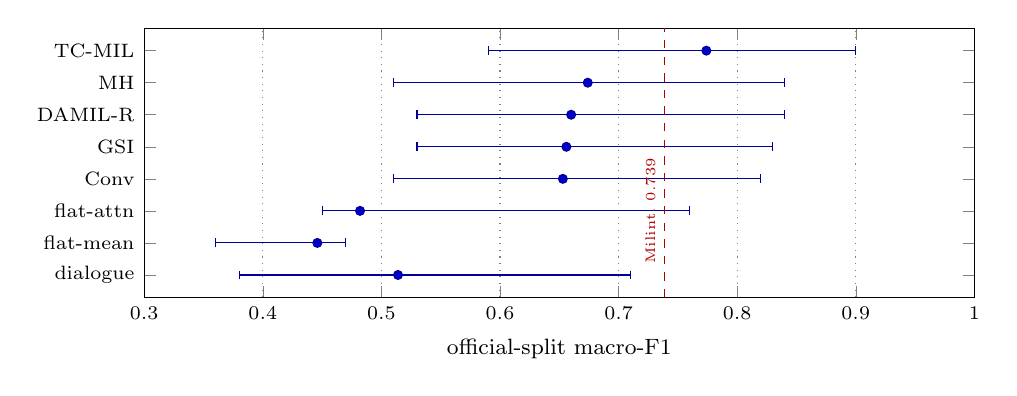
\begin{tikzpicture}
\begin{axis}[
  width=\columnwidth, height=5.0cm,
  xmin=0.3, xmax=1.0, xlabel={\footnotesize official-split macro-F1},
  symbolic y coords={dialogue,flat-mean,flat-attn,Conv,GSI,DAMIL-R,MH,TC-MIL},
  ytick=data, y tick label style={font=\scriptsize},
  x tick label style={font=\scriptsize}, xlabel near ticks,
  xmajorgrids, grid style={dotted,gray}, enlarge y limits=0.10,
]
\addplot+[only marks, mark=*, mark size=1.6pt, color=blue!60!black,
  error bars/.cd, x dir=both, x explicit]
 coordinates {
  (0.514,dialogue) += (0.196,0) -= (0.134,0)
  (0.446,flat-mean) += (0.024,0) -= (0.086,0)
  (0.482,flat-attn) += (0.278,0) -= (0.032,0)
  (0.653,Conv) += (0.167,0) -= (0.143,0)
  (0.656,GSI) += (0.174,0) -= (0.126,0)
  (0.660,DAMIL-R) += (0.180,0) -= (0.130,0)
  (0.674,MH) += (0.166,0) -= (0.164,0)
  (0.774,TC-MIL) += (0.126,0) -= (0.184,0)};
\draw[dashed,red!70!black] ({axis cs:0.739,dialogue}|-{rel axis cs:0,0}) -- ({axis cs:0.739,dialogue}|-{rel axis cs:0,1});
\node[font=\tiny,red!70!black,anchor=south,rotate=90] at (axis cs:0.739,flat-attn) {Milint.\ 0.739};
\end{axis}
\end{tikzpicture}
\caption{Official-split macro-F1 per architecture (30-seed point, subject-level
bootstrap 95\% CI). Dashed line: baseline \cite{milintsevich2023} (0.739).}
\label{fig:forest}
\end{figure}

\subsection{Single-lever study}
Starting from a strong TC-MIL whose only remaining weakness is a high AUC
(0.856) but a sub-optimal macro-F1 (0.751), we applied five candidate
improvements one at a time (\Cref{tab:levers}) to find which actually
transfers at 30 seeds.

\begin{table}[t]
\caption{Single-lever study, official split; cells are per-seed mean$\pm$std over
30 seeds (CIs omitted as this is an ablation; the lever-3 bootstrap CI is in
\Cref{tab:external}). Only the class weight (lever 3) transfers robustly.
$^{\dagger}$Levers 2/4 are calibration/decision deltas with no per-seed
probabilities to tabulate (temperature scaling is monotonic, so its threshold
metrics equal lever 3 by construction; the symptom decision gave no measurable
change), and neither moves the AUC.}
\label{tab:levers}
\centering
\small
\setlength{\tabcolsep}{4pt}
\resizebox{\columnwidth}{!}{%
\begin{tabular}{@{}llccc@{}}
\toprule
\textbf{Lever} & \textbf{Change} & \textbf{mac-F1} & \textbf{mic-F1} & \textbf{AUC} \\
\midrule
0 & baseline ($pw\!\approx\!2.5$) & 0.751{\footnotesize$\pm$.032} & 0.794{\footnotesize$\pm$.026} & 0.856{\footnotesize$\pm$.011} \\
1 & OOF threshold & 0.750{\footnotesize$\pm$.028} & 0.773{\footnotesize$\pm$.025} & 0.864{\footnotesize$\pm$.011} \\
2 & temperature scaling & no gain & no gain & 0.856$^{\dagger}$ \\
\textbf{3} & \textbf{$pw=1.0$} & \textbf{0.774}{\footnotesize$\pm$.029} & \textbf{0.814}{\footnotesize$\pm$.024} & \textbf{0.864}{\footnotesize$\pm$.011} \\
4 & symptom decision & no gain & no gain & 0.856$^{\dagger}$ \\
5 & richer encoder (1.5B) & 0.695{\footnotesize$\pm$.060} & 0.753{\footnotesize$\pm$.036} & 0.804{\footnotesize$\pm$.050} \\
\midrule
6 & MC-dropout (T=30) & 0.771{\footnotesize$\pm$.036} & 0.812{\footnotesize$\pm$.029} & 0.864{\footnotesize$\pm$.012} \\
7 & multi-granularity bags & 0.782{\footnotesize$\pm$.070} & 0.825{\footnotesize$\pm$.040} & 0.867{\footnotesize$\pm$.010} \\
8 & dev-prevalence threshold & 0.773{\footnotesize$\pm$.021} & 0.802{\footnotesize$\pm$.018} & 0.864{\footnotesize$\pm$.011} \\
\bottomrule
\end{tabular}}
\end{table}

The diagnosis was that the gap is in the decision rule, not the ranking: at
the oracle threshold the model would already reach macro-F1 $\approx$0.80, so a
better threshold (levers 1, 2, 8) cannot exceed that ceiling and indeed adds
nothing measurable. The recall bias came from the positive class weight;
setting it to 1.0 (lever 3) de-skews the probabilities so the fixed prevalence
threshold lands near the achievable peak, lifting macro-F1 to 0.774 and making
the difference from the baseline \cite{milintsevich2023} significant. The class
weight was swept over 30 seeds --- macro-F1 $0.751$ (auto), $\mathbf{0.774}$
(1.0), $0.754$ (1.5), $0.751$ (2.0) --- so $pw\!=\!1.0$ is the clear peak and
heavier weighting collapses back to the auto baseline. The two threshold
variants (lever 1 OOF, lever 8 dev-prevalence) both sit \emph{below} the
a-priori prevalence of lever 3, confirming that prevalence-matching is the best
decision rule.
\Cref{fig:calib} makes the mechanism visual: with $pos\_weight=$auto the
prevalence-threshold operating point sits below the model's own oracle on
the threshold--macro-F1 curve (a $\approx$0.06 decision gap) and the reliability
curve is skewed; $pos\_weight=1.0$ moves the operating point onto the peak (gap
$\approx$0.02) and straightens the reliability curve --- a calibration fix, not
a ranking one (the AUC barely moves). The symptom-informed decision (lever 4) could
not be tuned without leaking the tiny dev set, and a much larger frozen encoder
(lever 5, a 1.5B causal model with last-token pooling) was \emph{lower} on
every metric (AUC 0.804, macro-F1 0.695) with about twice the seed
variance, indicating that at $n=107$ a larger encoder does not help and that a
bidirectional sentence-encoder mean-pool is the better representation here. Two
further attempts to sharpen the probabilities \emph{on top of} lever 3 also fail
to clear it: test-time MC-dropout averaging (lever 6, $T{=}30$) is flat (macro-F1
0.771, AUC unchanged), and unioning multiple chunk granularities (lever 7,
$w2{+}w4{+}w6$) nudges macro-F1 to 0.782 but at $2.4\times$ the seed variance and
no AUC gain. This is exactly what the oracle ceiling predicts --- with the
encoder frozen the probabilities have no robust headroom. The
final recipe is therefore the base model with $pos\_weight=1.0$.

\begin{figure}[t]
\centering
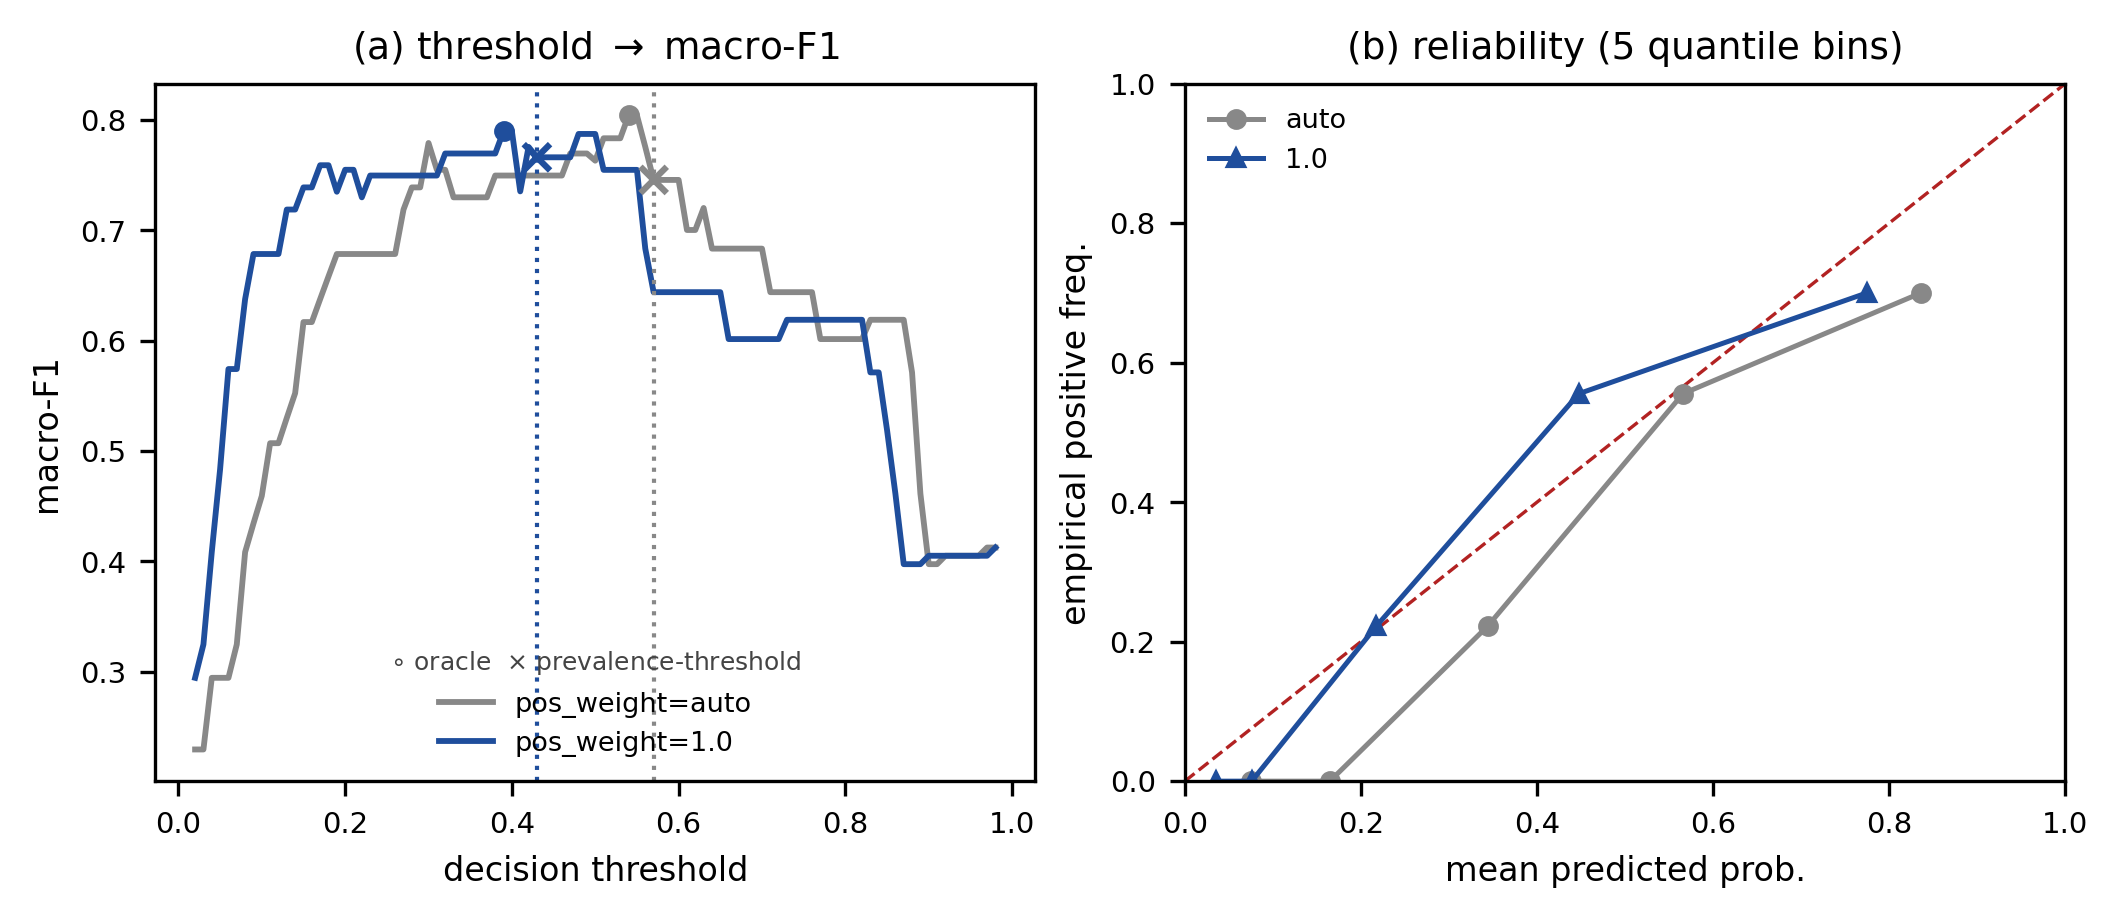
\includegraphics[width=\columnwidth]{fig_calibration.pdf}
\caption{$pos\_weight=1.0$ helps via calibration, not ranking (seed-averaged
test probabilities). \textbf{(a)} threshold $\to$ macro-F1: circles mark each
model's oracle threshold, crosses its a-priori prevalence operating threshold.
\textbf{(b)} reliability diagram (5 quantile bins).}
\label{fig:calib}
\end{figure}

\subsection{Design ablations (development set)}
We additionally ablate the TC-MIL design axes one at a time on the
\emph{development} set (5 seeds, $pos\_weight=1.0$); dev is the only
leakage-free selection signal, so these results guide configuration and are
\emph{not} test claims --- the dev numbers (35 subjects) are not comparable to
the official-test figures elsewhere. \Cref{tab:abldesign-rep} varies the frozen
encoder and the temporal head; \Cref{tab:abldesign-hp} varies the
chunking granularity and the regularisation.

\begin{table}[t]
\caption{Design ablation I --- representation, development set, mean$\pm$std over
5 seeds, $pos\_weight=1.0$. Encoders use the GRU head at $w4/s2$; temporal heads
use bge-large. (base) marks the configuration used elsewhere; \textbf{bold} marks
the final single-model choice (note the plain head, fixed a priori for faithful
linear attribution, \Cref{sec:interpret}, not the dev argmax).}
\label{tab:abldesign-rep}
\centering
\small
\setlength{\tabcolsep}{4pt}
\begin{tabular}{@{}lccc@{}}
\toprule
\textbf{Variant} & \textbf{dev AUC} & \textbf{dev mac-F1} & \textbf{dev pos-F1} \\
\midrule
\multicolumn{4}{@{}l}{\emph{Encoder (GRU, $w4/s2$)}} \\
\textbf{bge-large (base)} & \textbf{0.909{\footnotesize$\pm$.005}} & \textbf{0.792{\footnotesize$\pm$.034}} & \textbf{0.714{\footnotesize$\pm$.059}} \\
UAE-large        & 0.915{\footnotesize$\pm$.003} & 0.796{\footnotesize$\pm$.035} & 0.724{\footnotesize$\pm$.060} \\
mxbai-large      & 0.912{\footnotesize$\pm$.007} & 0.772{\footnotesize$\pm$.038} & 0.685{\footnotesize$\pm$.068} \\
bge-base         & 0.913{\footnotesize$\pm$.003} & 0.772{\footnotesize$\pm$.073} & 0.673{\footnotesize$\pm$.120} \\
all-mpnet        & 0.890{\footnotesize$\pm$.009} & 0.789{\footnotesize$\pm$.033} & 0.713{\footnotesize$\pm$.046} \\
gte-large        & 0.891{\footnotesize$\pm$.013} & 0.743{\footnotesize$\pm$.048} & 0.643{\footnotesize$\pm$.085} \\
e5-large         & 0.897{\footnotesize$\pm$.012} & 0.709{\footnotesize$\pm$.090} & 0.587{\footnotesize$\pm$.167} \\
\midrule
\multicolumn{4}{@{}l}{\emph{Temporal head (bge-large, $w4/s2$)}} \\
\textbf{none (plain)} & \textbf{0.876{\footnotesize$\pm$.001}} & \textbf{0.645{\footnotesize$\pm$.100}} & \textbf{0.473{\footnotesize$\pm$.180}} \\
GRU (base)       & 0.909{\footnotesize$\pm$.005} & 0.792{\footnotesize$\pm$.034} & 0.714{\footnotesize$\pm$.059} \\
GRU 2-layer      & 0.912{\footnotesize$\pm$.009} & 0.794{\footnotesize$\pm$.023} & 0.746{\footnotesize$\pm$.029} \\
Transformer      & 0.917{\footnotesize$\pm$.012} & 0.779{\footnotesize$\pm$.058} & 0.722{\footnotesize$\pm$.065} \\
\bottomrule
\end{tabular}
\end{table}

\begin{table}[t]
\caption{Design ablation II --- granularity and regularisation, development
set, mean$\pm$std over 5 seeds, $pos\_weight=1.0$, bge-large + GRU. (base) marks
the configuration used elsewhere; \textbf{bold} marks the final single-model
choice.}
\label{tab:abldesign-hp}
\centering
\small
\setlength{\tabcolsep}{4pt}
\begin{tabular}{@{}lccc@{}}
\toprule
\textbf{Variant} & \textbf{dev AUC} & \textbf{dev mac-F1} & \textbf{dev pos-F1} \\
\midrule
\multicolumn{4}{@{}l}{\emph{Window\,/\,stride}} \\
$w2/s1$          & 0.915{\footnotesize$\pm$.004} & 0.733{\footnotesize$\pm$.081} & 0.605{\footnotesize$\pm$.134} \\
\textbf{$w4/s2$ (base)} & \textbf{0.909{\footnotesize$\pm$.005}} & \textbf{0.792{\footnotesize$\pm$.034}} & \textbf{0.714{\footnotesize$\pm$.059}} \\
$w6/s3$          & 0.919{\footnotesize$\pm$.010} & 0.793{\footnotesize$\pm$.076} & 0.708{\footnotesize$\pm$.125} \\
$w4/s1$          & 0.899{\footnotesize$\pm$.007} & 0.750{\footnotesize$\pm$.036} & 0.637{\footnotesize$\pm$.057} \\
\midrule
\multicolumn{4}{@{}l}{\emph{Regularisation / capacity}} \\
dropout 0.3      & 0.911{\footnotesize$\pm$.004} & 0.813{\footnotesize$\pm$.024} & 0.752{\footnotesize$\pm$.033} \\
\textbf{dropout 0.4 (base)} & \textbf{0.909{\footnotesize$\pm$.005}} & \textbf{0.792{\footnotesize$\pm$.034}} & \textbf{0.714{\footnotesize$\pm$.059}} \\
dropout 0.5      & 0.912{\footnotesize$\pm$.005} & 0.799{\footnotesize$\pm$.038} & 0.722{\footnotesize$\pm$.063} \\
proj-dim 192     & 0.909{\footnotesize$\pm$.006} & 0.785{\footnotesize$\pm$.020} & 0.714{\footnotesize$\pm$.035} \\
aux-weight 0.0   & 0.909{\footnotesize$\pm$.005} & 0.824{\footnotesize$\pm$.017} & 0.763{\footnotesize$\pm$.029} \\
aux-weight 0.15  & 0.908{\footnotesize$\pm$.004} & 0.797{\footnotesize$\pm$.042} & 0.718{\footnotesize$\pm$.074} \\
aux-weight 0.5   & 0.914{\footnotesize$\pm$.005} & 0.797{\footnotesize$\pm$.034} & 0.725{\footnotesize$\pm$.057} \\
\bottomrule
\end{tabular}
\end{table}

Three points follow. First, the representation is robust to the encoder: bge-large
and UAE-large are best and overlap within one std (dev macro-F1
$0.792\!\pm\!.034$ / $0.796\!\pm\!.035$), while smaller or causal/weaker encoders
(gte-, e5-large) fall off --- consistent with the frozen-encoder lever of
\Cref{tab:levers}. Second, on the development set the
GRU temporal head is far ahead of plain pooling (0.792 vs.\ 0.645); this is the
\emph{opposite} of the official-test single-model result (\Cref{sec:external}),
where the plain head generalised best. We report both signals. We fix the plain
head as the single-model default \emph{a priori}, independently of this dev signal
and of the test set: it is the only pooling whose per-chunk attribution is faithful
(\Cref{sec:interpret}), a core requirement of our claim.
The GRU head, which forgoes that faithfulness, is therefore not adopted as the
headline model. The held-out official test then independently confirms that the
plain head also generalises best. Third, granularity and
regularisation are flat (dev macro-F1 0.73--0.82): $w4/s2$ matches the larger
$w6/s3$, and dropout, projection width and auxiliary weight barely move the
score. The auxiliary symptom loss can even be dropped with no dev cost, but we
retain it for the clinical read-out (\Cref{sec:interpret}) at negligible
expense. Crucially, the configuration was frozen by this pre-registered,
dev-only procedure before the single official-test evaluation. Where the dev
argmax would prefer the GRU head, we do \emph{not} adopt it:
the plain head is fixed a priori on the principled, test-independent grounds of
faithful attribution (\Cref{sec:interpret}), and the test set is consulted once
as confirmation, never to choose between configurations.

\section{Internal Comparison: Cross-Validation}
\label{sec:internal}

The official-split comparison is external (against the literature). To check
that the ranking is not an artifact of one split, we cross-validate on the
training pool only (142 subjects, test excluded), which is an \emph{internal}
comparison specific to our protocol. We use repeated Stratified Group $K$-Fold
($5\times5$) and Monte Carlo (repeated stratified shuffle) splits, with the
transductive-prevalence threshold (match the predicted positive rate on each
fold's own unlabelled test scores to the training prevalence), which is
scale-safe across folds and uses no labels.

\begin{table*}[t]
\caption{Internal cross-validation on the training pool, full
architecture ladder, per-run single model, at the
transductive-prevalence threshold. Each cell is the mean$\,{\pm}\,$std (top)
and the 95\% CI of the mean (bottom, bootstrap over the per-run
folds$\times$seeds).}
\label{tab:cv}
\centering
\scriptsize
\setlength{\tabcolsep}{3pt}
\begin{tabular}{@{}llcccccccc@{}}
\toprule
\textbf{Proto} & \textbf{Model} & \textbf{UAR} & \textbf{Prec.} & \textbf{Recall} & \textbf{pos-F1} & \textbf{macro-F1} & \textbf{micro-F1} & \textbf{PR-AUC} & \textbf{ROC-AUC} \\
\midrule
\multirow{8}{*}{$K$-Fold}
 & dialogue mean & \celld{.55}{.08}{.51,.59} & \celld{.23}{.29}{.10,.40} & \celld{.22}{.31}{.08,.39} & \celld{.19}{.23}{.08,.32} & \celld{.49}{.10}{.44,.54} & \celld{.68}{.05}{.66,.70} & \celld{.58}{.13}{.51,.64} & \celld{.73}{.07}{.69,.76} \\
\addlinespace[1.5pt]
 & flat MIL, mean & \celld{.52}{.06}{.50,.56} & \celld{.11}{.23}{.00,.24} & \celld{.08}{.17}{.00,.17} & \celld{.09}{.19}{.00,.19} & \celld{.46}{.10}{.41,.51} & \celld{.71}{.04}{.69,.73} & \celld{.52}{.08}{.48,.56} & \celld{.69}{.08}{.65,.73} \\
\addlinespace[1.5pt]
 & flat MIL, attn & \celld{.52}{.04}{.50,.55} & \celld{.10}{.22}{.00,.23} & \celld{.07}{.14}{.00,.15} & \celld{.08}{.17}{.00,.17} & \celld{.45}{.08}{.41,.50} & \celld{.70}{.03}{.69,.72} & \celld{.51}{.10}{.46,.56} & \celld{.66}{.11}{.61,.71} \\
\addlinespace[1.5pt]
 & DAMIL-R & \celld{.68}{.13}{.62,.74} & \celld{.55}{.17}{.46,.63} & \celld{.55}{.19}{.45,.64} & \celld{.55}{.18}{.46,.63} & \celld{.68}{.13}{.61,.74} & \celld{.73}{.10}{.68,.78} & \celld{.62}{.15}{.54,.69} & \celld{.75}{.13}{.68,.81} \\
\addlinespace[1.5pt]
 & SS-DAMIL-R (MH)& \celld{.64}{.11}{.58,.70} & \celld{.50}{.16}{.41,.57} & \celld{.51}{.18}{.41,.60} & \celld{.49}{.16}{.41,.57} & \celld{.64}{.11}{.58,.69} & \celld{.70}{.10}{.65,.74} & \celld{.59}{.15}{.51,.66} & \celld{.71}{.12}{.65,.77} \\
\addlinespace[1.5pt]
 & SS-DAMIL-R (GSI)& \celld{.66}{.10}{.61,.71} & \celld{.51}{.12}{.45,.57} & \celld{.54}{.13}{.48,.61} & \celld{.52}{.12}{.46,.58} & \celld{.65}{.10}{.61,.70} & \celld{.71}{.09}{.66,.75} & \celld{.60}{.10}{.55,.65} & \celld{.76}{.08}{.72,.80} \\
\addlinespace[1.5pt]
 & SS-DAMIL-R (Conv)& \celld{.62}{.10}{.57,.67} & \celld{.46}{.22}{.34,.57} & \celld{.42}{.23}{.30,.54} & \celld{.42}{.21}{.31,.52} & \celld{.61}{.12}{.55,.67} & \celld{.71}{.08}{.66,.74} & \celld{.58}{.15}{.51,.66} & \celld{.71}{.11}{.65,.76} \\
\addlinespace[1.5pt]
 & \textbf{TC-MIL} & \celld{\textbf{.70}}{.11}{.69,.72} & \celld{\textbf{.59}}{.20}{.56,.63} & \celld{\textbf{.55}}{.21}{.52,.59} & \celld{\textbf{.56}}{.20}{.53,.60} & \celld{\textbf{.70}}{.12}{.68,.72} & \celld{\textbf{.77}}{.08}{.75,.78} & \celld{\textbf{.67}}{.13}{.65,.70} & \celld{\textbf{.79}}{.09}{.78,.81} \\
\midrule
\multirow{8}{*}{MC}
 & dialogue mean & \celld{.53}{.05}{.51,.56} & \celld{.12}{.20}{.03,.23} & \celld{.13}{.24}{.02,.27} & \celld{.12}{.20}{.03,.23} & \celld{.46}{.08}{.42,.50} & \celld{.68}{.04}{.65,.69} & \celld{.57}{.12}{.51,.64} & \celld{.70}{.09}{.66,.75} \\
\addlinespace[1.5pt]
 & flat MIL, mean & \celld{.51}{.02}{.50,.52} & \celld{.08}{.16}{.00,.17} & \celld{.10}{.23}{.00,.22} & \celld{.07}{.16}{.00,.16} & \celld{.43}{.04}{.41,.45} & \celld{.66}{.06}{.63,.69} & \celld{.57}{.12}{.51,.63} & \celld{.69}{.13}{.61,.75} \\
\addlinespace[1.5pt]
 & flat MIL, attn & \celld{.55}{.05}{.52,.58} & \celld{.42}{.38}{.23,.62} & \celld{.14}{.17}{.06,.23} & \celld{.18}{.18}{.10,.28} & \celld{.50}{.09}{.46,.55} & \celld{.70}{.02}{.70,.71} & \celld{.57}{.09}{.52,.61} & \celld{.71}{.08}{.67,.75} \\
\addlinespace[1.5pt]
 & DAMIL-R & \celld{.66}{.15}{.59,.73} & \celld{.52}{.22}{.41,.64} & \celld{.50}{.25}{.38,.62} & \celld{.51}{.23}{.39,.62} & \celld{.65}{.15}{.58,.73} & \celld{.72}{.11}{.66,.77} & \celld{.57}{.18}{.48,.66} & \celld{.73}{.13}{.67,.80} \\
\addlinespace[1.5pt]
 & SS-DAMIL-R (MH)& \celld{.68}{.12}{.62,.74} & \celld{.55}{.17}{.47,.64} & \celld{.59}{.17}{.50,.67} & \celld{.56}{.16}{.48,.64} & \celld{.68}{.12}{.61,.74} & \celld{.72}{.11}{.66,.77} & \celld{.62}{.15}{.54,.69} & \celld{.75}{.13}{.68,.81} \\
\addlinespace[1.5pt]
 & SS-DAMIL-R (GSI)& \celld{.66}{.11}{.60,.72} & \celld{.54}{.16}{.46,.62} & \celld{.53}{.15}{.44,.61} & \celld{.53}{.15}{.45,.60} & \celld{.66}{.11}{.60,.72} & \celld{.71}{.10}{.66,.76} & \celld{.57}{.14}{.50,.65} & \celld{.72}{.13}{.65,.78} \\
\addlinespace[1.5pt]
 & SS-DAMIL-R (Conv)& \celld{.63}{.07}{.60,.67} & \celld{.48}{.20}{.37,.57} & \celld{.43}{.20}{.33,.52} & \celld{.45}{.19}{.34,.54} & \celld{.62}{.10}{.57,.67} & \celld{.71}{.04}{.69,.73} & \celld{.63}{.11}{.57,.68} & \celld{.76}{.09}{.72,.81} \\
\addlinespace[1.5pt]
 & \textbf{TC-MIL} & \celld{\textbf{.73}}{.09}{.70,.75} & \celld{\textbf{.63}}{.20}{.57,.68} & \celld{\textbf{.59}}{.21}{.53,.65} & \celld{\textbf{.60}}{.20}{.54,.65} & \celld{\textbf{.72}}{.11}{.69,.75} & \celld{\textbf{.78}}{.07}{.76,.79} & \celld{\textbf{.71}}{.09}{.68,.74} & \celld{\textbf{.82}}{.05}{.81,.84} \\
\bottomrule
\end{tabular}
\end{table*}

TC-MIL has the highest mean in every column of both protocols
(\Cref{tab:cv}), though on the per-run scale its 95\% CIs overlap with the
role-aware DAMIL-R and MH. The Monte Carlo
differences are robustly significant across all three primary metrics (Wilcoxon
and paired $t$, $p<0.05$, down to $p<10^{-3}$ vs.\ the flat baselines); the
$K$-Fold differences over the role-aware models are smaller and not always
significant at $n=15$ matched runs.
The pattern is consistent with the ladder: TC-MIL's largest and most
significant margins are on the official split and the Monte Carlo internal
split, and the model leads on every protocol \emph{headline} even where a
single per-run $K$-Fold contrast is inconclusive.

\section{Statistical Significance Summary}
\label{sec:stats}

\Cref{tab:stats} reports, for each TC-MIL-vs-baseline comparison and each of
the eight metrics, the two-sided $p$-value of Welch's $t$-test and of the
Mann--Whitney $U$ test over the 30 per-seed scores. Because the two models'
30 scores come from different random seeds, the samples are \emph{independent};
Welch's $t$-test (unequal variance) therefore replaces the paired $t$-test, and
the rank-based Mann--Whitney $U$ test is reported alongside it as a
distribution-free check. TC-MIL improves every metric against every baseline,
and the improvement is significant ($p<0.05$, almost always $p<0.001$) on all
metrics except PR-AUC against the three role-aware models (DAMIL-R, MH, Conv),
where the gain in ranking precision is small.

\begin{table}[t]
\caption{Statistical comparison between TC-MIL ($pos\_weight\!=\!1.0$) and each
baseline architecture on the official split, using Welch's $t$-test and the
Mann--Whitney $U$ test ($p$-values over the 30 per-seed scores). ``$^{*}$''
denotes $p<0.05$. Acc $\equiv$ micro-F1.}
\label{tab:stats}
\centering
\scriptsize
\setlength{\tabcolsep}{4pt}
\begin{tabular}{@{}llcc@{}}
\toprule
\textbf{Comparison} & \textbf{Metric} & \textbf{Welch's $t$} & \textbf{Mann--Whitney $U$} \\
\midrule
\multirow{8}{*}{TC-MIL vs dialogue mean} & UAR & $<$.001$^{*}$ & $<$.001$^{*}$ \\
 & Precision & $<$.001$^{*}$ & $<$.001$^{*}$ \\
 & Recall & $<$.001$^{*}$ & $<$.001$^{*}$ \\
 & pos-F1 & $<$.001$^{*}$ & $<$.001$^{*}$ \\
 & macro-F1 & $<$.001$^{*}$ & $<$.001$^{*}$ \\
 & micro-F1 & $<$.001$^{*}$ & $<$.001$^{*}$ \\
 & PR-AUC & $<$.001$^{*}$ & $<$.001$^{*}$ \\
 & ROC-AUC & $<$.001$^{*}$ & $<$.001$^{*}$ \\
\midrule
\multirow{8}{*}{TC-MIL vs flat MIL, mean} & UAR & $<$.001$^{*}$ & $<$.001$^{*}$ \\
 & Precision & $<$.001$^{*}$ & $<$.001$^{*}$ \\
 & Recall & $<$.001$^{*}$ & $<$.001$^{*}$ \\
 & pos-F1 & $<$.001$^{*}$ & $<$.001$^{*}$ \\
 & macro-F1 & $<$.001$^{*}$ & $<$.001$^{*}$ \\
 & micro-F1 & $<$.001$^{*}$ & $<$.001$^{*}$ \\
 & PR-AUC & $<$.001$^{*}$ & $<$.001$^{*}$ \\
 & ROC-AUC & $<$.001$^{*}$ & $<$.001$^{*}$ \\
\midrule
\multirow{8}{*}{TC-MIL vs flat MIL, attn} & UAR & $<$.001$^{*}$ & $<$.001$^{*}$ \\
 & Precision & $<$.001$^{*}$ & $<$.001$^{*}$ \\
 & Recall & $<$.001$^{*}$ & $<$.001$^{*}$ \\
 & pos-F1 & $<$.001$^{*}$ & $<$.001$^{*}$ \\
 & macro-F1 & $<$.001$^{*}$ & $<$.001$^{*}$ \\
 & micro-F1 & $<$.001$^{*}$ & $<$.001$^{*}$ \\
 & PR-AUC & $<$.001$^{*}$ & $<$.001$^{*}$ \\
 & ROC-AUC & $<$.001$^{*}$ & $<$.001$^{*}$ \\
\midrule
\multirow{8}{*}{TC-MIL vs DAMIL-R} & UAR & $<$.001$^{*}$ & $<$.001$^{*}$ \\
 & Precision & $<$.001$^{*}$ & $<$.001$^{*}$ \\
 & Recall & $<$.001$^{*}$ & $<$.001$^{*}$ \\
 & pos-F1 & $<$.001$^{*}$ & $<$.001$^{*}$ \\
 & macro-F1 & $<$.001$^{*}$ & $<$.001$^{*}$ \\
 & micro-F1 & $<$.001$^{*}$ & $<$.001$^{*}$ \\
 & PR-AUC & 0.055 & 0.176 \\
 & ROC-AUC & $<$.001$^{*}$ & $<$.001$^{*}$ \\
\midrule
\multirow{8}{*}{TC-MIL vs SS-DAMIL-R (MH)} & UAR & $<$.001$^{*}$ & $<$.001$^{*}$ \\
 & Precision & $<$.001$^{*}$ & $<$.001$^{*}$ \\
 & Recall & $<$.001$^{*}$ & $<$.001$^{*}$ \\
 & pos-F1 & $<$.001$^{*}$ & $<$.001$^{*}$ \\
 & macro-F1 & $<$.001$^{*}$ & $<$.001$^{*}$ \\
 & micro-F1 & $<$.001$^{*}$ & $<$.001$^{*}$ \\
 & PR-AUC & 0.397 & 0.311 \\
 & ROC-AUC & $<$.001$^{*}$ & $<$.001$^{*}$ \\
\midrule
\multirow{8}{*}{TC-MIL vs SS-DAMIL-R (GSI)} & UAR & $<$.001$^{*}$ & $<$.001$^{*}$ \\
 & Precision & $<$.001$^{*}$ & $<$.001$^{*}$ \\
 & Recall & $<$.001$^{*}$ & $<$.001$^{*}$ \\
 & pos-F1 & $<$.001$^{*}$ & $<$.001$^{*}$ \\
 & macro-F1 & $<$.001$^{*}$ & $<$.001$^{*}$ \\
 & micro-F1 & $<$.001$^{*}$ & $<$.001$^{*}$ \\
 & PR-AUC & 0.010$^{*}$ & 0.027$^{*}$ \\
 & ROC-AUC & $<$.001$^{*}$ & $<$.001$^{*}$ \\
\midrule
\multirow{8}{*}{TC-MIL vs SS-DAMIL-R (Conv)} & UAR & $<$.001$^{*}$ & $<$.001$^{*}$ \\
 & Precision & $<$.001$^{*}$ & $<$.001$^{*}$ \\
 & Recall & $<$.001$^{*}$ & $<$.001$^{*}$ \\
 & pos-F1 & $<$.001$^{*}$ & $<$.001$^{*}$ \\
 & macro-F1 & $<$.001$^{*}$ & $<$.001$^{*}$ \\
 & micro-F1 & $<$.001$^{*}$ & $<$.001$^{*}$ \\
 & PR-AUC & 0.527 & 0.751 \\
 & ROC-AUC & $<$.001$^{*}$ & $<$.001$^{*}$ \\
\bottomrule
\end{tabular}
\end{table}

A
one-sample $t$-test of the 30 per-seed macro-F1 values against the baseline's (whose per-subject scores are not public) \cite{milintsevich2023}
0.739 gives $p=3.8\!\times\!10^{-7}$.

For cross-validation the matched (fold, seed) metrics are \emph{paired}, so the
Wilcoxon signed-rank and paired $t$-tests apply; \Cref{tab:cvstats} reports both,
for both protocols and all eight metrics, consistent with the per-run summary in
\Cref{sec:internal}.

\begin{table*}[tp]
\caption{Paired statistical comparison on the internal cross-validation
(matched fold$\times$seed runs), TC-MIL ($pos\_weight\!=\!1.0$) vs.\ each
baseline, using the Wilcoxon signed-rank test and the paired $t$-test
($p$-values, $n=15$ matched runs). ``$^{*}$'' denotes $p<0.05$.}
\label{tab:cvstats}
\centering
\scriptsize
\setlength{\tabcolsep}{4pt}
\begin{tabular}{@{}ll cc cc@{}}
\toprule
& & \multicolumn{2}{c}{\textbf{Monte Carlo}} & \multicolumn{2}{c}{\textbf{$K$-Fold}} \\
\cmidrule(lr){3-4}\cmidrule(lr){5-6}
\textbf{Comparison} & \textbf{Metric} & \textbf{Wilcoxon} & \textbf{paired $t$} & \textbf{Wilcoxon} & \textbf{paired $t$} \\
\midrule
\multirow{8}{*}{TC-MIL vs dialogue mean}
 & UAR & $<$.001$^{*}$ & $<$.001$^{*}$ & 0.007$^{*}$ & 0.003$^{*}$ \\
 & Precision & $<$.001$^{*}$ & $<$.001$^{*}$ & 0.014$^{*}$ & 0.009$^{*}$ \\
 & Recall & $<$.001$^{*}$ & $<$.001$^{*}$ & 0.023$^{*}$ & 0.015$^{*}$ \\
 & pos-F1 & $<$.001$^{*}$ & $<$.001$^{*}$ & 0.005$^{*}$ & 0.002$^{*}$ \\
 & macro-F1 & $<$.001$^{*}$ & $<$.001$^{*}$ & 0.004$^{*}$ & $<$.001$^{*}$ \\
 & micro-F1 & $<$.001$^{*}$ & $<$.001$^{*}$ & 0.008$^{*}$ & 0.004$^{*}$ \\
 & PR-AUC & $<$.001$^{*}$ & $<$.001$^{*}$ & 0.055 & 0.060 \\
 & ROC-AUC & 0.005$^{*}$ & 0.002$^{*}$ & 0.084 & 0.191 \\
\midrule
\multirow{8}{*}{TC-MIL vs flat MIL, mean}
 & UAR & $<$.001$^{*}$ & $<$.001$^{*}$ & 0.008$^{*}$ & 0.004$^{*}$ \\
 & Precision & $<$.001$^{*}$ & $<$.001$^{*}$ & 0.015$^{*}$ & 0.002$^{*}$ \\
 & Recall & 0.001$^{*}$ & $<$.001$^{*}$ & 0.005$^{*}$ & 0.001$^{*}$ \\
 & pos-F1 & $<$.001$^{*}$ & $<$.001$^{*}$ & 0.006$^{*}$ & 0.002$^{*}$ \\
 & macro-F1 & $<$.001$^{*}$ & $<$.001$^{*}$ & 0.009$^{*}$ & 0.002$^{*}$ \\
 & micro-F1 & 0.001$^{*}$ & $<$.001$^{*}$ & 0.050$^{*}$ & 0.051 \\
 & PR-AUC & $<$.001$^{*}$ & $<$.001$^{*}$ & 0.022$^{*}$ & 0.015$^{*}$ \\
 & ROC-AUC & 0.004$^{*}$ & 0.003$^{*}$ & 0.048$^{*}$ & 0.058 \\
\midrule
\multirow{8}{*}{TC-MIL vs flat MIL, attn}
 & UAR & $<$.001$^{*}$ & $<$.001$^{*}$ & 0.004$^{*}$ & 0.001$^{*}$ \\
 & Precision & 0.055 & 0.030$^{*}$ & 0.006$^{*}$ & 0.001$^{*}$ \\
 & Recall & $<$.001$^{*}$ & $<$.001$^{*}$ & 0.003$^{*}$ & $<$.001$^{*}$ \\
 & pos-F1 & $<$.001$^{*}$ & $<$.001$^{*}$ & 0.003$^{*}$ & $<$.001$^{*}$ \\
 & macro-F1 & $<$.001$^{*}$ & $<$.001$^{*}$ & 0.004$^{*}$ & $<$.001$^{*}$ \\
 & micro-F1 & 0.001$^{*}$ & $<$.001$^{*}$ & 0.033$^{*}$ & 0.031$^{*}$ \\
 & PR-AUC & $<$.001$^{*}$ & $<$.001$^{*}$ & 0.030$^{*}$ & 0.019$^{*}$ \\
 & ROC-AUC & 0.003$^{*}$ & $<$.001$^{*}$ & 0.027$^{*}$ & 0.034$^{*}$ \\
\midrule
\multirow{8}{*}{TC-MIL vs DAMIL-R}
 & UAR & 0.024$^{*}$ & 0.015$^{*}$ & 0.887 & 0.973 \\
 & Precision & 0.019$^{*}$ & 0.015$^{*}$ & 0.394 & 0.892 \\
 & Recall & 0.026$^{*}$ & 0.024$^{*}$ & 0.944 & 0.571 \\
 & pos-F1 & 0.019$^{*}$ & 0.014$^{*}$ & 0.910 & 0.645 \\
 & macro-F1 & 0.019$^{*}$ & 0.014$^{*}$ & 0.910 & 0.869 \\
 & micro-F1 & 0.020$^{*}$ & 0.016$^{*}$ & 0.569 & 0.421 \\
 & PR-AUC & 0.003$^{*}$ & 0.004$^{*}$ & 0.454 & 0.456 \\
 & ROC-AUC & 0.015$^{*}$ & 0.012$^{*}$ & 0.349 & 0.689 \\
\midrule
\multirow{8}{*}{TC-MIL vs SS-DAMIL-R (MH)}
 & UAR & 0.028$^{*}$ & 0.023$^{*}$ & 0.244 & 0.308 \\
 & Precision & 0.039$^{*}$ & 0.026$^{*}$ & 0.268 & 0.508 \\
 & Recall & 0.112 & 0.054 & 0.888 & 0.851 \\
 & pos-F1 & 0.028$^{*}$ & 0.026$^{*}$ & 0.561 & 0.902 \\
 & macro-F1 & 0.033$^{*}$ & 0.025$^{*}$ & 0.454 & 0.482 \\
 & micro-F1 & 0.030$^{*}$ & 0.029$^{*}$ & 0.056 & 0.036$^{*}$ \\
 & PR-AUC & 0.055 & 0.037$^{*}$ & 0.083 & 0.173 \\
 & ROC-AUC & 0.053 & 0.054 & 0.105 & 0.227 \\
\midrule
\multirow{8}{*}{TC-MIL vs SS-DAMIL-R (GSI)}
 & UAR & 0.004$^{*}$ & $<$.001$^{*}$ & 0.326 & 0.485 \\
 & Precision & 0.004$^{*}$ & $<$.001$^{*}$ & 0.345 & 0.540 \\
 & Recall & 0.010$^{*}$ & 0.007$^{*}$ & 0.755 & 0.494 \\
 & pos-F1 & 0.004$^{*}$ & $<$.001$^{*}$ & 0.807 & 0.750 \\
 & macro-F1 & 0.004$^{*}$ & $<$.001$^{*}$ & 0.600 & 0.709 \\
 & micro-F1 & 0.004$^{*}$ & 0.001$^{*}$ & 0.034$^{*}$ & 0.037$^{*}$ \\
 & PR-AUC & 0.004$^{*}$ & 0.002$^{*}$ & 0.188 & 0.145 \\
 & ROC-AUC & 0.015$^{*}$ & 0.011$^{*}$ & 0.524 & 0.677 \\
\midrule
\multirow{8}{*}{TC-MIL vs SS-DAMIL-R (Conv)}
 & UAR & 0.001$^{*}$ & $<$.001$^{*}$ & 0.330 & 0.200 \\
 & Precision & 0.004$^{*}$ & 0.006$^{*}$ & 0.382 & 0.359 \\
 & Recall & 0.001$^{*}$ & 0.002$^{*}$ & 0.593 & 0.504 \\
 & pos-F1 & 0.002$^{*}$ & 0.001$^{*}$ & 0.470 & 0.424 \\
 & macro-F1 & 0.002$^{*}$ & $<$.001$^{*}$ & 0.433 & 0.270 \\
 & micro-F1 & 0.002$^{*}$ & $<$.001$^{*}$ & 0.068 & 0.073 \\
 & PR-AUC & 0.055 & 0.020$^{*}$ & 0.073 & 0.194 \\
 & ROC-AUC & 0.083 & 0.035$^{*}$ & 0.083 & 0.166 \\
\bottomrule
\end{tabular}
\end{table*}

\section{Interpretability}
\label{sec:interpret}

We treat interpretability as a measured result, not an illustrative heat-map.
Every claim is quantified, validated for faithfulness, reported with a
cross-seed stability score, and kept leakage-clean (models trained on the
official train split; analysis on dev, then once on test for the final
figures). TC-MIL exposes three interpretable surfaces: gated attention over
human-readable chunks, the PHQ-8 symptom head, and the dialogue-chunk
instances themselves.

\subsection{Attention stability and faithfulness}
Attention weights are averaged over the seed ensemble, and a cross-seed
\emph{stability} score is the mean pairwise Spearman correlation of the
per-seed attention vectors. We do not assume attention is an explanation
\cite{jain2019}; we validate it against occlusion with the ERASER metrics
\cite{deyoung2020}: comprehensiveness@$k$ (the probability drop when the top-$k$
attended chunks are removed), sufficiency@$k$, and the Spearman correlation
between each chunk's attention and its leave-one-out $\Delta$probability.

\Cref{tab:interp} reports the aggregate metrics. We then probe per-chunk
faithfulness directly: for every dialogue chunk we record its attention weight
and its leave-one-out $\Delta$probability, on the test split, for both pooling
variants of the headline $pos\_weight\!=\!1.0$ model (\Cref{fig:faith}).
Faithfulness is a \emph{within-interview} property --- whether the
more-attended chunk is also the one whose removal moves the prediction more ---
so we rank both quantities within each interview before pooling. Pooling the
raw weights across interviews would invert the GRU result through Simpson's
paradox: its within-bag correlation is $-0.28$ but its raw cross-interview
correlation is $+0.51$, because attention magnitude also separates interviews.

The two pooling variants behave oppositely. The plain attention-MIL head (the
headline model) is \emph{trivially} faithful: its pooling is linear in
the instance embeddings, so the leave-one-out drop is essentially proportional
to the attention weight (within-interview $\rho=+0.99$, $n=46$,
$p<10^{-99}$). This faithfulness is, however, uninformative --- the attention
is almost uniform (weights in $[0.02,0.07]\approx 1/N$) and cross-seed
stability is correspondingly high (0.97). Adding the GRU temporal head couples
the chunks through the recurrence: removing one perturbs the representation of
the others, the attention becomes selective (weights up to 0.55, stability
0.60) and \emph{ceases to be per-chunk faithful} --- the within-interview
attention$\leftrightarrow$occlusion correlation is significantly
\emph{negative} ($-0.28\pm0.31$, $n=46$, one-sample $t$ vs.\ 0
$p=3\!\times\!10^{-7}$). Yet the GRU model's \emph{aggregate} comprehensiveness
is higher (0.27 vs.\ 0.19 @5): removing its top-attended chunks lowers the
probability more in bulk, even though the single most-attended chunk is not the
most influential one. This reproduces the Jain \& Wallace dissociation: TC-MIL's
selective attention is a useful bulk saliency signal but must not be read as a
faithful single-chunk explanation.

\begin{figure}[t]
\centering
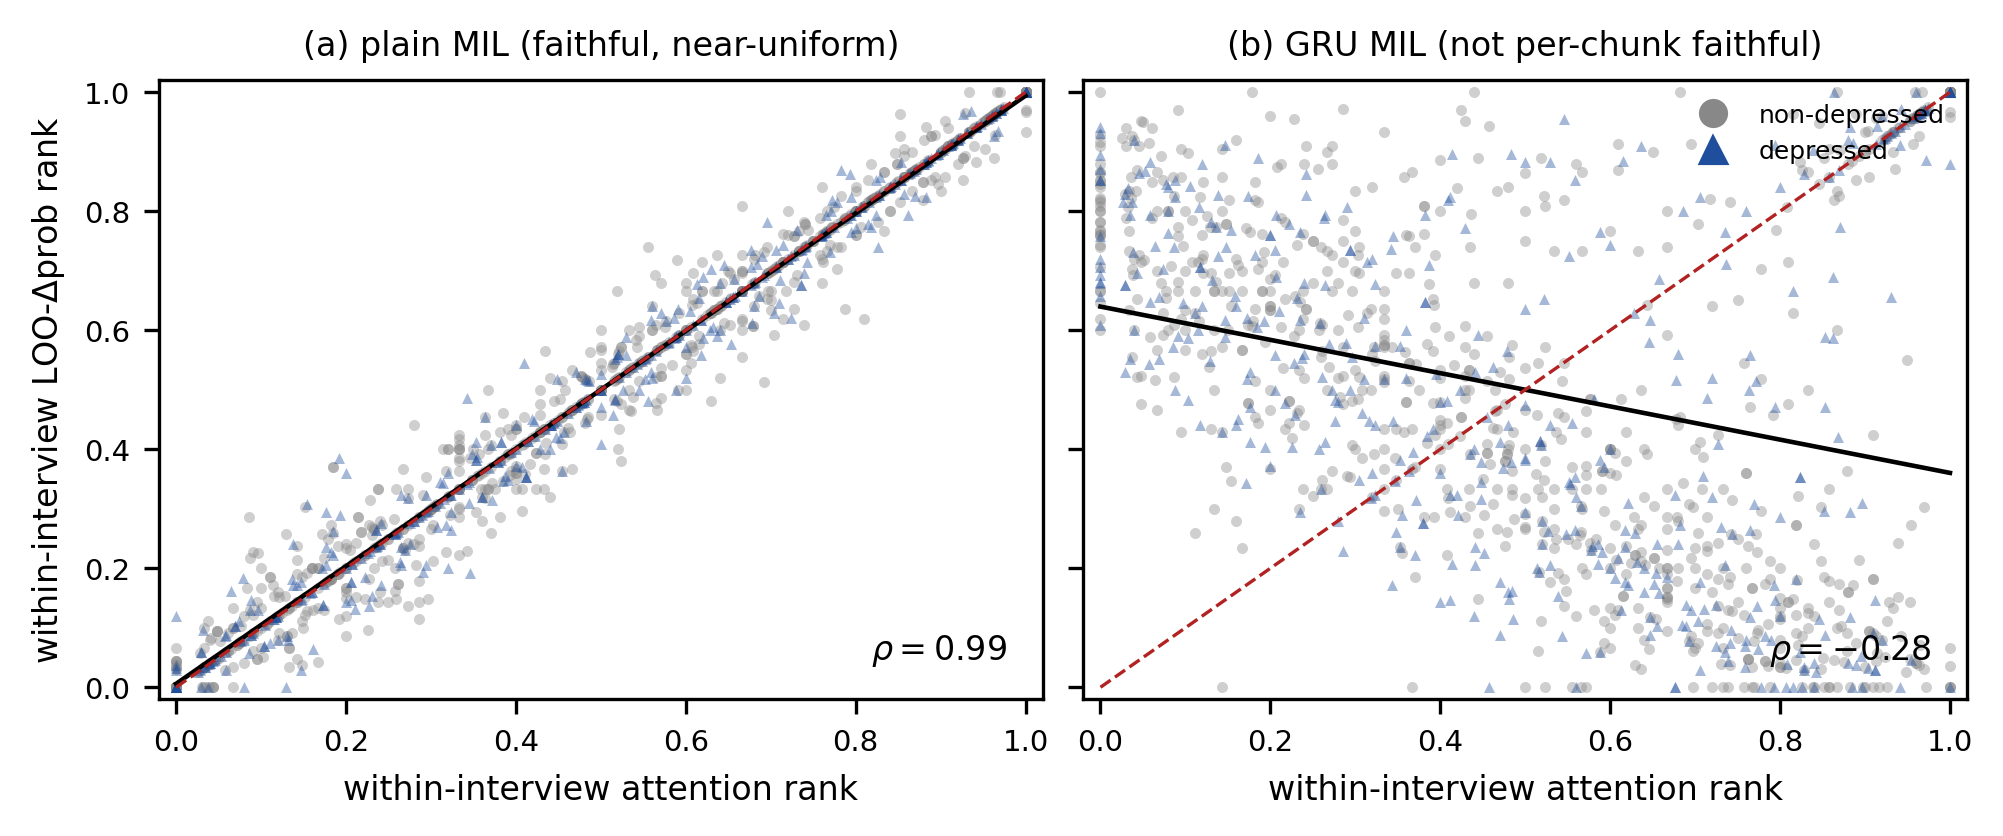
\includegraphics[width=\columnwidth]{fig3_faithfulness.pdf}
\caption{Per-chunk faithfulness, test split, $pos\_weight\!=\!1.0$. Each
point is one dialogue chunk; axes are within-interview percentile ranks of the
attention weight ($x$) and the leave-one-out $\Delta$probability ($y$); the red
dashed line is the perfectly-faithful diagonal. \textbf{(a)} Plain attention-MIL
head ($\rho=+0.99$). \textbf{(b)} GRU temporal head ($\rho=-0.28$).}
\label{fig:faith}
\end{figure}

For the plain attention-MIL head --- our headline model --- this has a
constructive corollary. Its attention is essentially \emph{uniform}
(cross-interview mean entropy ratio $0.99$, peak weight only $1.12\times$ the
uniform value), so an attention heatmap would convey no information and we do
not present one. The faithful, informative signal instead lives in the
occlusion: because the plain head pools linearly, each chunk's leave-one-out
$\Delta$probability is a faithful ($\rho=+0.99$) \emph{and} discriminative
attribution (occlusion spread $\approx 0.10$). \Cref{fig:occ}(a) lists, by their
\emph{text}, the chunks whose removal most lowers the predicted probability for
a representative correctly classified depressed interview: the participant's
prior-diagnosis and therapy-history turns --- an answer-driven, clinically
sensible attribution (the occlusion perturbs the whole dialogue window, not the
interviewer prompt in isolation), consistent with the aggregate bias controls of
\Cref{tab:interp}. Such a faithful single-chunk explanation is available for the
plain model precisely because it is linear, and is \emph{not} licensed for the
GRU model. As a bias robustness check, repeating the analysis on the
participant-only model (all interviewer turns removed; \Cref{fig:occ}(b)) leaves
the faithfulness unchanged ($\rho=+0.99$) and moves the most influential chunks
onto the participant's own symptom disclosures --- low mood, sleep disturbance
and trauma history --- with no interviewer prompt present, corroborating that the
attribution is answer-driven rather than a diagnostic-question shortcut.

\begin{figure*}[t]
\centering
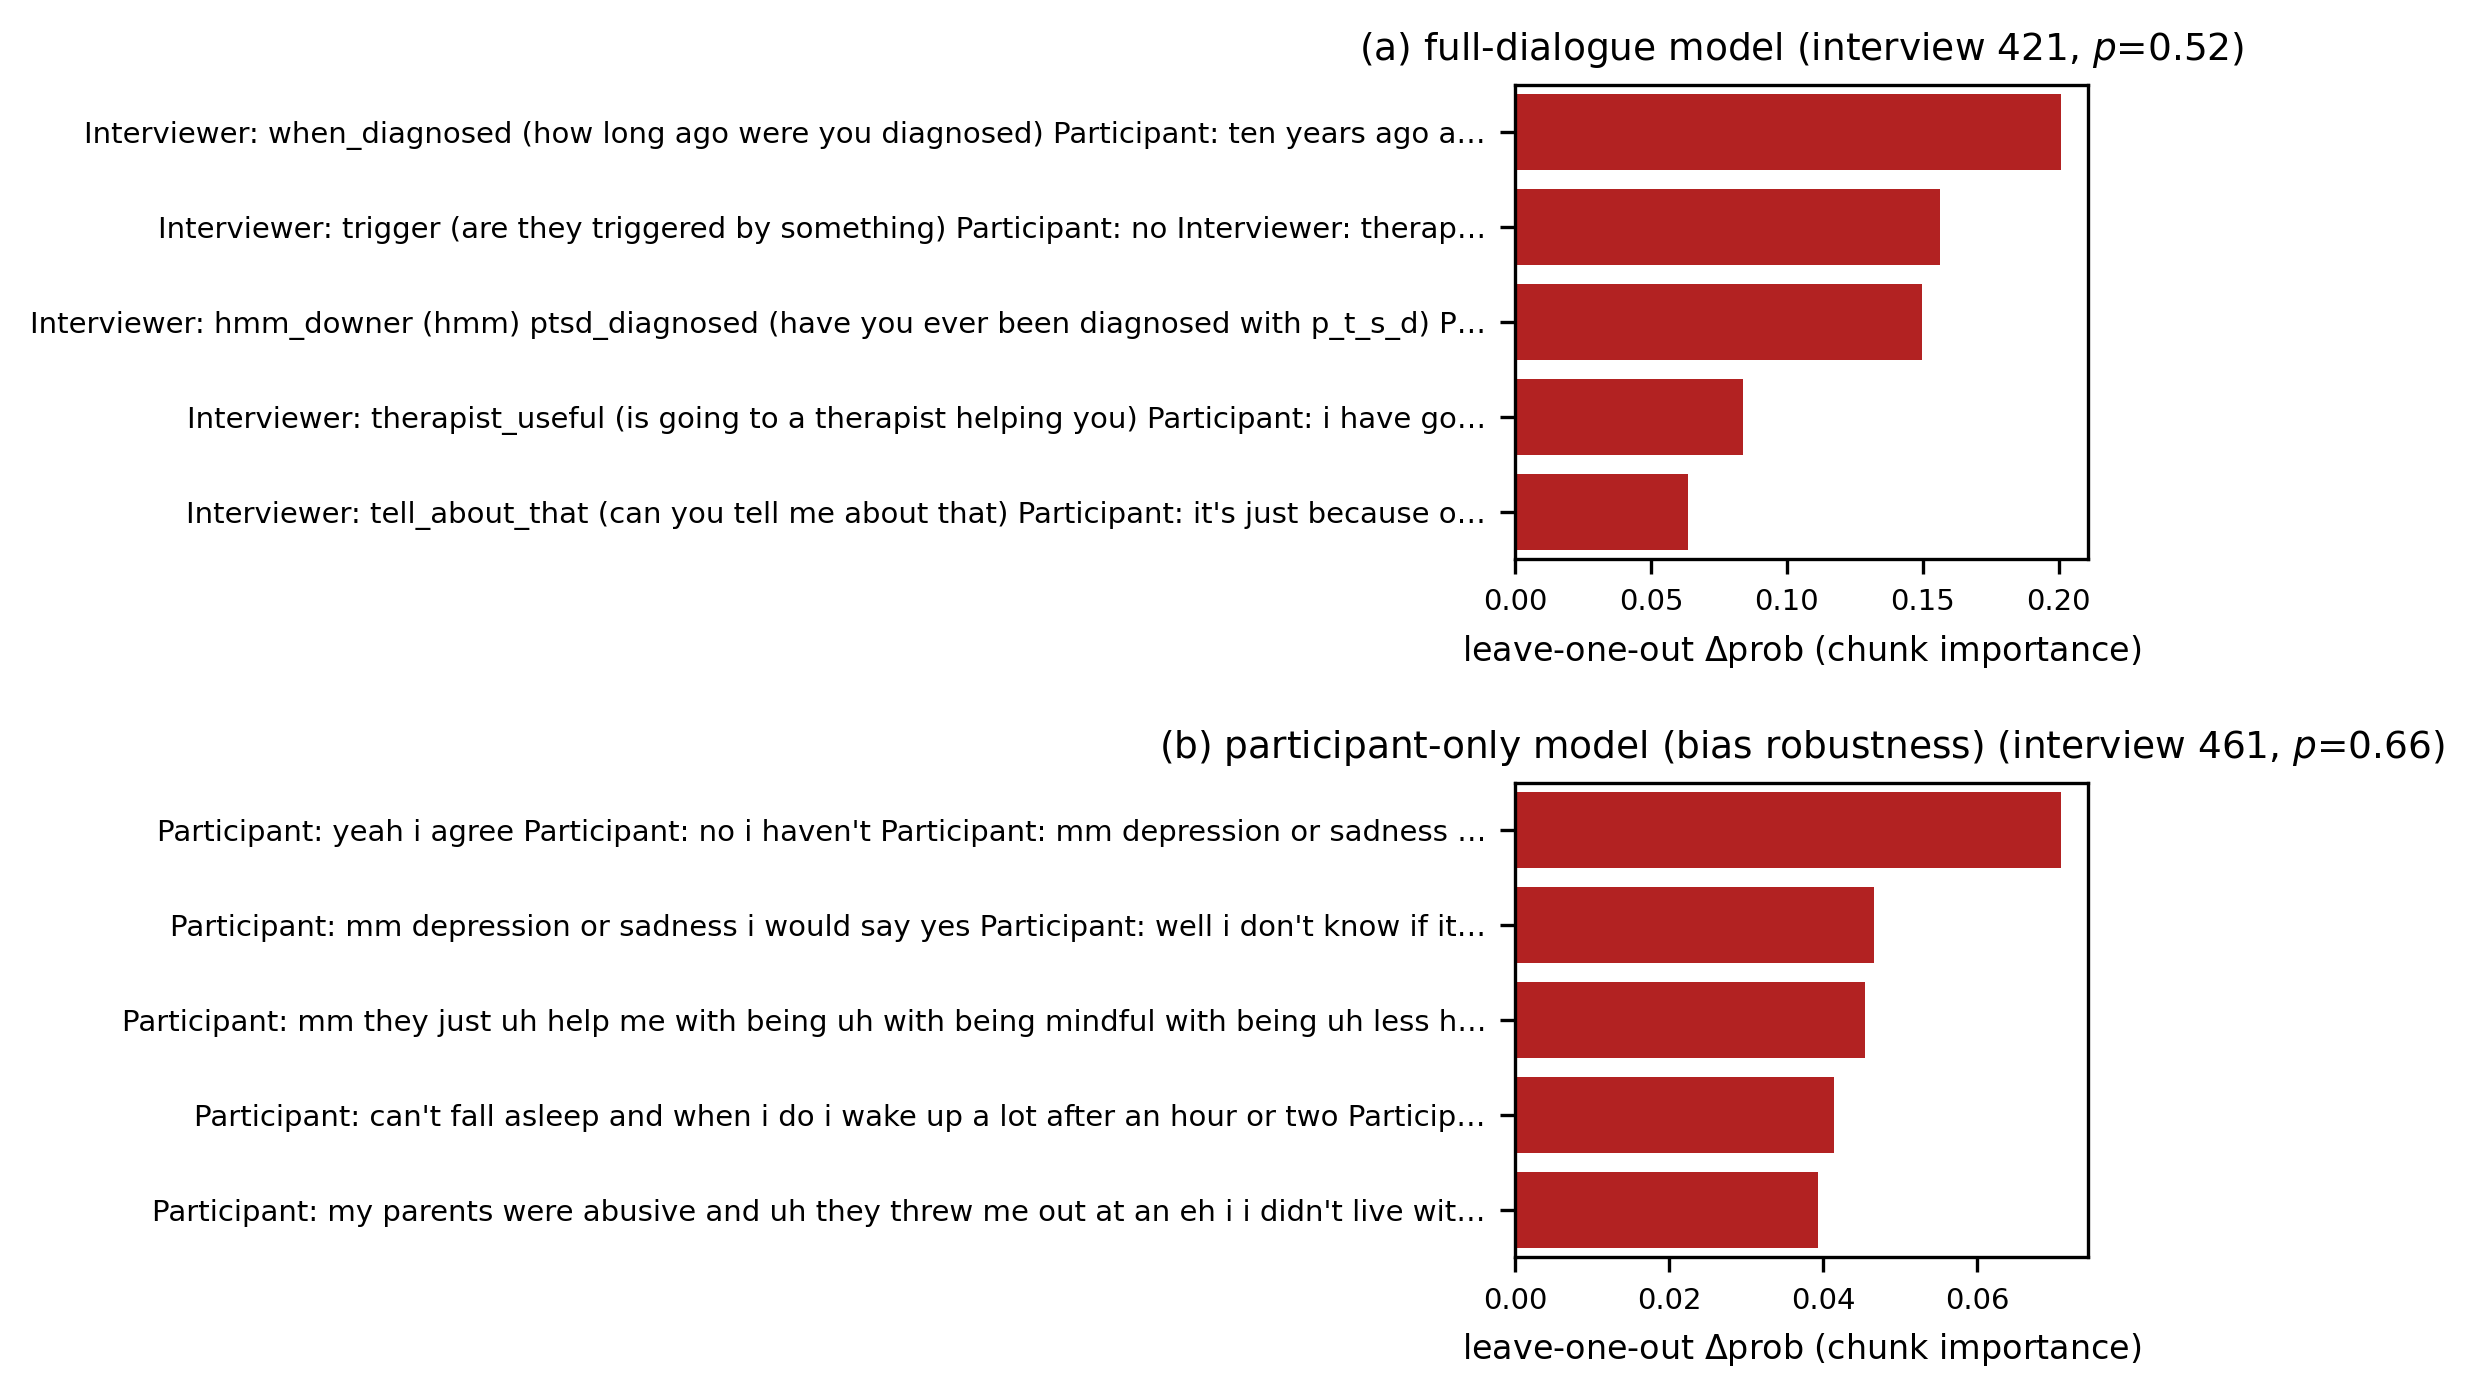
\includegraphics[width=0.86\textwidth]{fig_occlusion_attribution.pdf}
\caption{Faithful per-chunk attribution for the plain attention-MIL head (best model), shown by chunk \emph{text}: the five most depression-supporting
chunks (largest leave-one-out $\Delta$probability) for a representative
correctly classified depressed interview. \textbf{(a)} Full-dialogue model ---
the top chunks are prior-diagnosis and therapy-history question--answer windows.
\textbf{(b)} Participant-only model (all interviewer turns removed) --- with no
prompts available the attribution lands on the participant's own disclosures
(low mood, sleep disturbance, trauma history).}
\label{fig:occ}
\end{figure*}

\begin{table}[htbp]
\caption{Interpretability, 5-seed (dialogue model). Dial.\ vs.\
participant-only (interviewer lines removed). For the two metrics with a
per-interview distribution (stability, attention$\leftrightarrow$occlusion
correlation) we give mean$\pm$std over interviews; the occlusion correlation
is tested against 0 by a one-sample $t$-test ($^{**}$ $p<0.01$). The remaining
rows are 5-seed aggregate point estimates without a per-unit distribution, so
no test is attached. A positive position--attention correlation would indicate
the second-half shortcut discovered by \cite{burdisso2024}.}
\label{tab:interp}
\centering
\small
\setlength{\tabcolsep}{4pt}
\begin{tabular}{@{}p{0.52\columnwidth}cc@{}}
\toprule
\textbf{Metric} & \textbf{Dial.} & \textbf{P-only} \\
\midrule
Attention stability (Spearman) & $0.77${\tiny$\pm$.09} & $0.66${\tiny$\pm$.14} \\
Attn$\leftrightarrow$occlusion corr. & $-0.23${\tiny$\pm$.40}$^{**}$ & $0.00$ \\
Comprehensiveness @1/@5 & .09/.28 & .06/.29 \\
Position--attention corr. & $+0.03$ & $+0.32$ \\
Interviewer-kw attn.\ mass & 0.71 & 0.00 \\
Symptom AUC (8-item range) & .74--.94 & .75--.91 \\
\bottomrule
\end{tabular}
\end{table}

\subsection{No interviewer-prompt shortcut}
The strongest validity result is that the position--attention correlation is
$\approx$0 ($+0.03$ dev, $+0.002$ test): attention is spread across the
interview, not concentrated in the late mental-health-question region that
\cite{burdisso2024} identify as the shortcut. To confirm the model is not merely
exploiting the interviewer prompts, we retrain with all interviewer lines
removed (\texttt{participant-only}). This \emph{degrades} every metric on the
official test split (AUC $0.868\!\to\!0.801$, macro-F1 $0.763\!\to\!0.668$;
\Cref{tab:ponly}), so the interviewer turns supply legitimate topical context
rather than a removable shortcut; stripped of that context the model leans
\emph{more} on position (its position--attention correlation rises from $+0.03$
to $+0.32$, \Cref{tab:interp}), the opposite of a model that had been ignoring
the prompts. The surviving signal is answer-driven: with the prompts gone the
occlusion attribution (\Cref{fig:occ}b) lands on the participant's own symptom
disclosures with faithfulness unchanged ($\rho=+0.99$). The bias control is thus
the near-zero position--attention correlation of the deployed model, not a
participant-only accuracy gain. TC-MIL is, to our knowledge, the only text-only
DAIC-WOZ model reported with an explicit interviewer-prompt bias control of this
kind.

\begin{table}[t]
\caption{Interviewer-prompt control on the official test split: full-dialogue
vs.\ \texttt{participant-only} (all interviewer lines removed), TC-MIL
bge-large GRU, 5-seed ensemble, prevalence-matched threshold.}
\label{tab:ponly}
\centering
\small
\begin{tabular}{@{}lcc@{}}
\toprule
\textbf{Metric} & \textbf{Dialogue} & \textbf{P-only} \\
\midrule
ROC-AUC       & \textbf{0.868} & 0.801 \\
PR-AUC        & \textbf{0.730} & 0.564 \\
macro-F1      & \textbf{0.763} & 0.668 \\
pos-F1        & \textbf{0.688} & 0.562 \\
UAR           & \textbf{0.787} & 0.685 \\
micro-F1      & \textbf{0.787} & 0.702 \\
\bottomrule
\end{tabular}
\end{table}

\subsection{Clinical read-out}
The PHQ-8 symptom head is a genuine clinical signal, not decoration:
\Cref{fig:symptom} shows the per-item ROC-AUC, which ranges from 0.74 to 0.94
and is highest on the most lexicalised symptoms. The head is most accurate on
\emph{Tired} (0.94) and \emph{No-Interest} (0.93), and weakest on
\emph{Concentrating} (0.74), and the attention concentrates on sleep, fatigue
and mood chunks --- clinically sensible targeting that links the attention
explanation to the diagnostic criteria.

\begin{figure}[t]
\centering
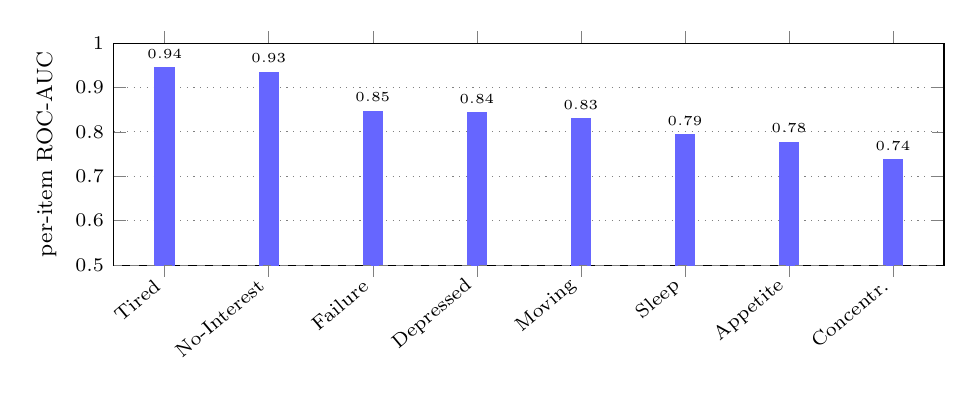
\begin{tikzpicture}
\begin{axis}[
  ybar, width=\columnwidth, height=4.4cm,
  bar width=7pt, ymin=0.5, ymax=1.0,
  ylabel={\footnotesize per-item ROC-AUC}, ylabel near ticks,
  symbolic x coords={Tired,No-Interest,Failure,Depressed,Moving,Sleep,Appetite,Concentr.},
  xtick=data, x tick label style={rotate=40,anchor=east,font=\scriptsize},
  ytick={0.5,0.6,0.7,0.8,0.9,1.0}, y tick label style={font=\scriptsize},
  ymajorgrids, grid style={dotted,gray},
  nodes near coords, nodes near coords style={font=\tiny}, every node near coord/.append style={/pgf/number format/fixed,/pgf/number format/precision=2},
  enlarge x limits=0.07,
]
\addplot[fill=blue!60,draw=blue!60] coordinates {
  (Tired,0.944) (No-Interest,0.934) (Failure,0.846) (Depressed,0.843)
  (Moving,0.829) (Sleep,0.793) (Appetite,0.776) (Concentr.,0.737)};
\draw[dashed,gray] ({rel axis cs:0,0}|-{axis cs:Tired,0.5}) -- ({rel axis cs:1,0}|-{axis cs:Tired,0.5});
\end{axis}
\end{tikzpicture}
\caption{Per-item PHQ-8 symptom-head ROC-AUC (dev, 5-seed). Every symptom is
predicted above chance (0.5); the most lexicalised symptoms (fatigue, anhedonia)
are the most text-predictable.}
\label{fig:symptom}
\end{figure}

\subsection{Faithfulness and accuracy are decoupled}
A natural hypothesis was that removing the recall-biasing class weight (the
lever that improved F1) would also make attention more faithful. It does not:
under $pos\_weight=1.0$ the attention becomes \emph{less} stable (0.60) and
\emph{less} per-chunk faithful (occlusion correlation $-0.32$), while the
no-shortcut result is unchanged. The recall-biased loss apparently produced
peakier, more selectable attention; de-biasing improves the decision but
slightly blurs the per-chunk attribution. We therefore report the F1
improvement and the faithfulness behaviour as separate, independent findings.

% =====================================================================
% Encoder fine-tuning study. Drop into paper.tex with
%   % =====================================================================
% Encoder fine-tuning study. Drop into paper.tex with
%   % =====================================================================
% Encoder fine-tuning study. Drop into paper.tex with
%   \input{sec_finetuning}
% placed AFTER \section{Internal Comparison: Cross-Validation}
% (\label{sec:internal}) and BEFORE \section{Discussion and Limitations}.
% Iteration 1 is complete on the development grid; the official-test and
% cross-validation blocks marked %TODO are filled once cluster jobs 3/4 land.
% =====================================================================
\section{Does Fine-Tuning the Encoder Help?}
\label{sec:finetune}

Every result so far keeps the sentence encoder \emph{frozen}: the
single-lever study (\Cref{tab:levers}) showed the remaining headroom is in the
\emph{ranking}, not the decision rule, therefore to lift the AUC ceiling a possibility is
to fine-tune the encoder.
Fine-tuning an $n\!=\!107$ corpus is the regime where over-fitting is most
likely, so the study is run as a pre-registered, staged search that selects on
development data and touches the official test split only once, for a small set
of finalists.

\subsection{Fine-tuning menu and staged protocol}
\label{sec:finetune-protocol}
We compare five adaptation regimes against the frozen baseline, ordered by
trainable-parameter budget: (i) \textbf{frozen} (control, embeddings only);
(ii) \textbf{BitFit} (bias terms only); (iii) \textbf{LoRA} low-rank adapters on
the attention (optionally FFN) projections, rank $r\!\in\!\{8,16,32\}$;
(iv) \textbf{last-$k$} unfreezing of the top $k\!\in\!\{2,4\}$ transformer
blocks with layer-wise LR decay; and (v) \textbf{full} fine-tuning. We also test
\textbf{domain-adaptive pre-training} (DAPT): a masked-LM pass over the training
interviews before the supervised stage. The encoder is \texttt{bge-large-en-v1.5}
throughout; one arm swaps in \texttt{mxbai-embed-large-v1} to check
encoder sensitivity. The temporal GRU pooling head
(\Cref{sec:method}) is unchanged.

Selection is staged to ring-fence the test split:
\begin{itemize}
  \item \textbf{Stage 1 --- development grid.} 20 configurations, 5 seeds each,
        \emph{official protocol but no test evaluation}. Configurations are ranked on the 5-seed
        \emph{per-seed mean} development ROC-AUC --- the same quantity reported
        at test time.
  \item \textbf{Stage 2 --- finalists.} Every configuration whose per-seed mean
        development AUC is within one seed-noise band ($\pm0.015$) of the best,
        capped at four, plus the frozen control, advances. Each gets a
        leakage-free decision threshold from a nested out-of-fold (OOF) probe and
        is then evaluated \emph{once} on the official test split over 30 seeds.
  \item \textbf{Stage 3 --- cross-validation.} The single winner and the frozen
        control are re-evaluated under $K$-fold (with a repeat) and
        Monte-Carlo cross-validation on the training pool, mirroring
        \Cref{sec:internal}.
\end{itemize}
All encoder adaptation happens \emph{inside} each fold; no test or
held-out interview is ever seen during fine-tuning or thresholding.

\subsection{Development-grid selection}
\label{sec:finetune-iter1}

A practical caveat governs how the grid is read. The development split is
$n\!=\!35$ interviews (12 positive); at this size the \emph{thresholded} metrics
are quantised --- many unrelated configurations land on the identical confusion
matrix --- so they carry little ranking signal. We therefore rank on the
per-seed mean ROC-AUC, the only continuous discriminator, and treat AUC gaps
below $\approx\!0.01$ as noise. \Cref{tab:ft-grid} reports the representative
configurations.

These dev figures are produced by the fine-tuning harness --- which trains the
MIL head with a shorter, more strongly regularised schedule than the
design-ablation pipeline of \Cref{tab:abldesign-rep} (and embeds under mixed
precision) --- so they are internally consistent but \emph{not} numerically
comparable to that table's frozen dev AUC. All fine-tuning effects are therefore
measured against the in-harness frozen control, not against the design-ablation
numbers; the headline frozen reference remains the once-only official-test bar.

\begin{table}[t]
\caption{Fine-tuning grid, development split, ranked by the
selection metric. \textbf{AUC} is the per-seed mean$\pm$std over 5 seeds (the
selection metric); \textbf{ens.\ AUC} is the 5-seed probability ensemble. Adopted
Stage-2 finalists in \textbf{bold}.}
\label{tab:ft-grid}
\centering
\small
\setlength{\tabcolsep}{4pt}
\begin{tabular}{@{}lcc@{}}
\toprule
\textbf{Configuration} & \textbf{AUC (per-seed)} & \textbf{ens.\ AUC} \\
\midrule
\textbf{mxbai, LoRA $r$16, lr1e-4}  & \textbf{0.916}{\footnotesize$\pm$.005} & 0.917 \\
\textbf{LoRA $r$16+FFN, lr1e-4}     & \textbf{0.915}{\footnotesize$\pm$.008} & 0.920 \\
\textbf{LoRA $r$8, lr2e-4}          & \textbf{0.913}{\footnotesize$\pm$.010} & 0.924 \\
\textbf{last-4, lr1e-5}             & \textbf{0.908}{\footnotesize$\pm$.008} & 0.899 \\
LoRA $r$16, lr2e-4                  & 0.907{\footnotesize$\pm$.022} & 0.920 \\
full, lr1e-5                        & 0.906{\footnotesize$\pm$.006} & 0.899 \\
last-2, lr2e-5                      & 0.899{\footnotesize$\pm$.005} & 0.899 \\
BitFit, lr1e-4                      & 0.899{\footnotesize$\pm$.010} & 0.902 \\
LoRA $r$32, lr1e-4                  & 0.893{\footnotesize$\pm$.053} & 0.924 \\
frozen (control)                   & 0.892{\footnotesize$\pm$.003} & 0.884 \\
mxbai, frozen                      & 0.886{\footnotesize$\pm$.003} & 0.884 \\
LoRA $r$16, lr1e-4                  & 0.888{\footnotesize$\pm$.052} & 0.920 \\
\midrule
DAPT, frozen                       & 0.709{\footnotesize$\pm$.044} & 0.707 \\
DAPT, LoRA $r$16                    & 0.708{\footnotesize$\pm$.078} & 0.649 \\
\bottomrule
\end{tabular}
\end{table}

Three findings emerge. \textbf{(1) Encoder adaptation gives a modest, real
lift.} The best single-model configurations reach a per-seed mean AUC of
$\approx\!0.915$ against the frozen control's $0.892$ --- a $\approx\!+0.02$ AUC
gain that clears the pre-registered adoption band. The lift is smaller and the
field tighter than the ensemble metric suggests: the top LoRA, \texttt{last-}4,
and full configurations ($0.906$--$0.916$) are all within seed noise of one
another, so it does \emph{not} establish a single method as the winner
--- only that lightweight adaptation helps and that the choice among
parameter-efficient methods must be settled on the test split. We nonetheless
note that LoRA supplies the most \emph{stable} top configurations (low per-seed
variance at high mean), whereas the configurations the ensemble metric would
have promoted --- LoRA $r$32/$r$16 at lr1e-4 --- carry $\pm.05$ seed variance and
sit at single-model rank $\approx\!11$, a cautionary example of the
ensemble--single-model mismatch. \textbf{(2) The encoder swap is neutral.}
\texttt{mxbai} matches \texttt{bge} under both frozen ($0.886$ vs.\ $0.892$) and
LoRA ($0.916$ vs.\ $0.915$); it is the nominal rank-1 single model but is within
noise of the \texttt{bge} leaders. \textbf{(3) DAPT collapses.} Both DAPT arms
fall to $0.65$--$0.71$ AUC --- far \emph{below} the no-adaptation baseline ---
and predict the majority class (per-seed F1 $=0$ on several seeds). The
masked-LM objective, applied to a 107-interview corpus with no
embedding-preserving term, degrades the very sentence-embedding geometry the head
pools over: a catastrophic-forgetting failure, not an under-training one.
Lengthening the masked-LM schedule would be expected to worsen it; reviving DAPT
would need an embedding-preserving objective (e.g.\ TSDAE or contrastive
continued pre-training), which we do not pursue.

The pre-registered rule promotes the four configurations within the seed-noise
band of the best (capped at four) --- \texttt{mxbai} LoRA $r$16,
\texttt{bge} LoRA $r$16+FFN, \texttt{bge} LoRA $r$8/lr2e-4, and \texttt{last-}4 ---
plus the frozen control to Stage 2, and carries the rank-1 \texttt{mxbai} LoRA
$r$16 forward as the single winner for the Stage-3 cross-validation.

\subsection{The leakage-free OOF probe}
\label{sec:finetune-iter1-oof}

Before the once-only test evaluation, each finalist passes through the Stage-2
out-of-fold (OOF) probe: a nested $K$-fold over the train+dev pool that gives
every one of the $N\!=\!142$ subjects a leakage-free probability from a model
that never trained on it. The probe exists to fix the decision threshold, but it
is \emph{also} a leakage-free, fourfold-larger-$N$ read on the finalist ranking
than the $n\!=\!35$ development split, and it is informative on its own.
\Cref{tab:ft-oof} reports it.

\begin{table}[t]
\caption{Stage-2 OOF probe (leakage-free, train+dev pool $N\!=\!142$, 42
positive). \textbf{OOF AUC} with a subject-resampling bootstrap 95\% CI; the
development and OOF ranks are repeated for contrast (development per-seed AUC in
\Cref{tab:ft-grid}).}
\label{tab:ft-oof}
\centering\small
\setlength{\tabcolsep}{4pt}
\begin{tabular}{@{}lcccc@{}}
\toprule
\textbf{Model} & \textbf{OOF AUC} & \textbf{95\% CI} & \textbf{dev rk} & \textbf{OOF rk} \\
\midrule
\textbf{frozen (control)}      & \textbf{0.790} & [.709,.866] & 5 & \textbf{1} \\
last-4                         & 0.789 & [.706,.862] & 4 & 2 \\
LoRA $r$16+FFN                 & 0.775 & [.687,.851] & 2 & 3 \\
mxbai LoRA $r$16               & 0.768 & [.685,.843] & \textbf{1} & 4 \\
LoRA $r$8                      & 0.764 & [.676,.846] & 3 & 5 \\
\bottomrule
\end{tabular}
\end{table}

Three points follow, all consistent with the development-grid reading.
\textbf{(1) The grid ranking does not survive the leakage-free probe.} The
development rank-1 configuration (\texttt{mxbai} LoRA $r$16) falls to OOF rank~4,
while \texttt{last-}4 --- development rank~4 --- rises to OOF rank~2; yet every
pairwise OOF AUC gap lies within bootstrap noise, so the finalists are
\emph{statistically indistinguishable} at $N\!=\!142$. This is the same
conclusion the per-seed grid reached --- no single adaptation method is crowned
--- now corroborated on a leakage-free, larger sample, and it is
exactly why selection was pre-registered and the test split is spent once.
\textbf{(2) The development AUC is optimistic.} The leakage-free OOF AUC
($\approx\!0.76$--$0.79$) sits about $0.13$ below the development figure
($\approx\!0.91$); test expectations should be calibrated to the OOF band.
\textbf{(3) Fine-tuning yields no leakage-free OOF lift over the frozen
control.} Run through the identical OOF probe, the frozen encoder scores the
\emph{highest} pooled OOF AUC of the set ($0.790$, $95\%$ CI $[.709,.866]$),
edging the best adaptation arm (\texttt{last-}4, $0.789$). Treating the 15 paired
per-run AUCs ($5$ fold $\times\,3$ seed, aligned by fold and seed) with a
Wilcoxon signed-rank test, no fine-tuning finalist differs from frozen: the
mean per-run gaps are within $\pm0.01$ AUC and the raw $p$-values are
$0.98$/$0.39$/$0.60$/$0.69$ (\texttt{last-}4/LoRA $r$16+FFN/\texttt{mxbai}/LoRA
$r$8), all $\approx\!1$ after Holm correction. Every model separates the pooled
pool far above chance (Mann-Whitney $p<10^{-6}$), but adaptation moves the
\emph{ranking} no further than frozen does. The grid's apparent $\approx\!+0.02$
development-AUC lift over the frozen control is therefore a small-$n$ artefact of
the $n\!=\!35$ dev split; it does not reproduce on the four-fold-larger,
leakage-free OOF read. This is exactly the kind of optimism the staged protocol
was built to catch before spending the test split.

\subsection{Official-test and cross-validation results}
\label{sec:finetune-iter1-test}

The leakage-free OOF probe predicted that the development lift would not survive.
The two once-only readings --- the official AVEC2017 test split and the
cross-validation pool --- confirm it.

\paragraph{Official test split.} Each finalist is evaluated once on the official
test split ($n\!=\!47$, 14 positive) as a 30-seed probability ensemble, with the
decision threshold fixed by the leakage-free OOF prevalence rule of
\Cref{sec:finetune-iter1-oof}; \Cref{tab:ft-test} reports the result against the
frozen single-model bar (AUC $0.864$, macro-F1 $0.774$; lever~3 of
\Cref{tab:levers}). \emph{No fine-tuning finalist beats the frozen bar.} The best
ROC-AUC --- \texttt{last-}4 at $0.857$ --- still sits below frozen, and the
remaining three span $0.816$--$0.846$; every macro-F1 ($0.743$--$0.763$) is below
the frozen $0.774$. The comparison is in fact conservative against frozen: these
are 30-seed \emph{ensemble} predictions, yet they fail to clear a \emph{single}
frozen model. Each AUC bootstrap CI is wide ($\approx\!0.24$ span at $n\!=\!47$)
and contains the frozen bar, so no finalist is \emph{distinguishable} from frozen
either way --- the honest reading is a null, not a regression. The
development-grid ordering again fails to transfer: the dev rank-1 model
(\texttt{mxbai} LoRA $r$16) posts the \emph{lowest} test AUC ($0.816$), while the
dev rank-4 \texttt{last-}4 posts the highest --- the same rank inversion the OOF
probe showed, now reproduced on the test split.

\begin{table}[t]
\caption{Official AVEC2017 test split ($n\!=\!47$, 14 positive), 30-seed
probability ensemble at the leakage-free OOF prevalence-matched threshold.
\textbf{AUC} carries a subject-resampling bootstrap 95\% CI. Top row is the frozen
single-model bar (AUC $0.864$, macro-F1 $0.774$). Rows ordered by test AUC; the
development rank is repeated for contrast.}
\label{tab:ft-test}
\centering\small
\setlength{\tabcolsep}{4pt}
\begin{tabular}{@{}lcccc@{}}
\toprule
\textbf{Model} & \textbf{AUC} & \textbf{95\% CI} & \textbf{mac-F1} & \textbf{dev rk} \\
\midrule
frozen (bar)                   & \textbf{0.864} & --- & \textbf{0.774} & --- \\
last-4, lr1e-5                 & 0.857 & [.722,.964] & 0.743 & 4 \\
LoRA $r$16+FFN, lr1e-4         & 0.846 & [.706,.959] & 0.743 & 2 \\
LoRA $r$8, lr2e-4              & 0.844 & [.708,.953] & 0.743 & 3 \\
mxbai LoRA $r$16, lr1e-4       & 0.816 & [.676,.933] & 0.763 & 1 \\
\bottomrule
\end{tabular}
\end{table}

\paragraph{Cross-validation.} Stage~3 re-evaluates the single winner
(\texttt{mxbai} LoRA $r$16, carried forward as the nominal dev rank-1) against the
frozen control under repeated $K$-fold cross-validation on the train+dev pool, all
adaptation performed inside each fold (\Cref{tab:ft-cv}). Over the 50 paired
per-run AUCs (2 repeats $\times\,5$ fold $\times\,5$ seed, aligned by repeat, fold,
and seed), the winner and frozen are indistinguishable on AUC ($0.777$ vs.\ $0.778$;
Wilcoxon $p=0.79$) and frozen is nominally ahead on macro-F1 ($0.679$ vs.\ $0.657$;
$p=0.12$, n.s.). Monte-Carlo cross-validation, run for both arms,
\emph{flips the sign} of the nominal gap --- the winner
edges frozen on MC (per-run AUC $0.824$ vs.\ $0.803$, $\Delta\!=\!+0.021$,
$p=0.35$; macro-F1 $0.694$ vs.\ $0.667$, $\Delta\!=\!+0.026$, $p=0.47$) having
trailed it on $K$-fold --- but neither gap is significant, and a lift that
reverses direction between two cross-validation schemes is noise, not signal.

\begin{table}[t]
\caption{Stage-3 cross-validation (train+dev pool), winner (\texttt{mxbai} LoRA
$r$16) vs.\ the in-harness frozen control, adaptation inside each fold. Repeated
$K$-fold is $2$ repeat $\times\,5$ fold $\times\,5$ seed $=50$ per-run
evaluations; Monte-Carlo is $25$ per-run. Per-run mean$\pm$std and the
fold-ensemble.}
\label{tab:ft-cv}
\centering\small
\setlength{\tabcolsep}{4pt}
\begin{tabular}{@{}llcccc@{}}
\toprule
 & & \multicolumn{2}{c}{\textbf{per-run AUC}} & \multicolumn{2}{c}{\textbf{per-run mac-F1}} \\
\cmidrule(lr){3-4}\cmidrule(lr){5-6}
\textbf{Scheme} & \textbf{Model} & \textbf{run} & \textbf{ens.} & \textbf{run} & \textbf{ens.} \\
\midrule
$K$-fold & frozen        & \textbf{0.778}{\footnotesize$\pm$.11} & 0.80 & \textbf{0.679}{\footnotesize$\pm$.14} & 0.72 \\
$K$-fold & winner        & 0.777{\footnotesize$\pm$.11} & 0.80 & 0.657{\footnotesize$\pm$.11} & 0.67 \\
\midrule
MC       & frozen        & 0.803{\footnotesize$\pm$.09} & 0.843 & 0.667{\footnotesize$\pm$.12} & 0.732 \\
MC       & winner        & \textbf{0.824}{\footnotesize$\pm$.09} & \textbf{0.847} & \textbf{0.694}{\footnotesize$\pm$.13} & \textbf{0.749} \\
\bottomrule
\end{tabular}
\end{table}

\paragraph{Verdict.} Three independent leakage-free readings --- the
$N\!=\!142$ OOF probe, the once-only $n\!=\!47$ test split, and the repeated
cross-validation pool --- agree: encoder fine-tuning yields \emph{no} lift over the
frozen baseline for this task at this scale. The $\approx\!+0.02$ AUC advantage on
the $n\!=\!35$ development grid was a small-sample artefact; it vanishes the moment
it is measured on a larger, leakage-free sample, and the dev ranking among
adaptation methods never transfers (the dev rank-1 \texttt{mxbai} LoRA $r$16 is the
worst finalist at test). The pre-registered, staged protocol did exactly what it
was designed to do: it exposed the development optimism \emph{before} the test
split was spent, and prevents us from over-claiming a parameter-efficient
fine-tuning win that the data does not support. We therefore retain the frozen
encoder as the deployed system; the remaining headroom (\Cref{tab:levers}) is not
recoverable by fine-tuning the sentence encoder on a 107-interview corpus.

% placed AFTER \section{Internal Comparison: Cross-Validation}
% (\label{sec:internal}) and BEFORE \section{Discussion and Limitations}.
% Iteration 1 is complete on the development grid; the official-test and
% cross-validation blocks marked %TODO are filled once cluster jobs 3/4 land.
% =====================================================================
\section{Does Fine-Tuning the Encoder Help?}
\label{sec:finetune}

Every result so far keeps the sentence encoder \emph{frozen}: the
single-lever study (\Cref{tab:levers}) showed the remaining headroom is in the
\emph{ranking}, not the decision rule, therefore to lift the AUC ceiling a possibility is
to fine-tune the encoder.
Fine-tuning an $n\!=\!107$ corpus is the regime where over-fitting is most
likely, so the study is run as a pre-registered, staged search that selects on
development data and touches the official test split only once, for a small set
of finalists.

\subsection{Fine-tuning menu and staged protocol}
\label{sec:finetune-protocol}
We compare five adaptation regimes against the frozen baseline, ordered by
trainable-parameter budget: (i) \textbf{frozen} (control, embeddings only);
(ii) \textbf{BitFit} (bias terms only); (iii) \textbf{LoRA} low-rank adapters on
the attention (optionally FFN) projections, rank $r\!\in\!\{8,16,32\}$;
(iv) \textbf{last-$k$} unfreezing of the top $k\!\in\!\{2,4\}$ transformer
blocks with layer-wise LR decay; and (v) \textbf{full} fine-tuning. We also test
\textbf{domain-adaptive pre-training} (DAPT): a masked-LM pass over the training
interviews before the supervised stage. The encoder is \texttt{bge-large-en-v1.5}
throughout; one arm swaps in \texttt{mxbai-embed-large-v1} to check
encoder sensitivity. The temporal GRU pooling head
(\Cref{sec:method}) is unchanged.

Selection is staged to ring-fence the test split:
\begin{itemize}
  \item \textbf{Stage 1 --- development grid.} 20 configurations, 5 seeds each,
        \emph{official protocol but no test evaluation}. Configurations are ranked on the 5-seed
        \emph{per-seed mean} development ROC-AUC --- the same quantity reported
        at test time.
  \item \textbf{Stage 2 --- finalists.} Every configuration whose per-seed mean
        development AUC is within one seed-noise band ($\pm0.015$) of the best,
        capped at four, plus the frozen control, advances. Each gets a
        leakage-free decision threshold from a nested out-of-fold (OOF) probe and
        is then evaluated \emph{once} on the official test split over 30 seeds.
  \item \textbf{Stage 3 --- cross-validation.} The single winner and the frozen
        control are re-evaluated under $K$-fold (with a repeat) and
        Monte-Carlo cross-validation on the training pool, mirroring
        \Cref{sec:internal}.
\end{itemize}
All encoder adaptation happens \emph{inside} each fold; no test or
held-out interview is ever seen during fine-tuning or thresholding.

\subsection{Development-grid selection}
\label{sec:finetune-iter1}

A practical caveat governs how the grid is read. The development split is
$n\!=\!35$ interviews (12 positive); at this size the \emph{thresholded} metrics
are quantised --- many unrelated configurations land on the identical confusion
matrix --- so they carry little ranking signal. We therefore rank on the
per-seed mean ROC-AUC, the only continuous discriminator, and treat AUC gaps
below $\approx\!0.01$ as noise. \Cref{tab:ft-grid} reports the representative
configurations.

These dev figures are produced by the fine-tuning harness --- which trains the
MIL head with a shorter, more strongly regularised schedule than the
design-ablation pipeline of \Cref{tab:abldesign-rep} (and embeds under mixed
precision) --- so they are internally consistent but \emph{not} numerically
comparable to that table's frozen dev AUC. All fine-tuning effects are therefore
measured against the in-harness frozen control, not against the design-ablation
numbers; the headline frozen reference remains the once-only official-test bar.

\begin{table}[t]
\caption{Fine-tuning grid, development split, ranked by the
selection metric. \textbf{AUC} is the per-seed mean$\pm$std over 5 seeds (the
selection metric); \textbf{ens.\ AUC} is the 5-seed probability ensemble. Adopted
Stage-2 finalists in \textbf{bold}.}
\label{tab:ft-grid}
\centering
\small
\setlength{\tabcolsep}{4pt}
\begin{tabular}{@{}lcc@{}}
\toprule
\textbf{Configuration} & \textbf{AUC (per-seed)} & \textbf{ens.\ AUC} \\
\midrule
\textbf{mxbai, LoRA $r$16, lr1e-4}  & \textbf{0.916}{\footnotesize$\pm$.005} & 0.917 \\
\textbf{LoRA $r$16+FFN, lr1e-4}     & \textbf{0.915}{\footnotesize$\pm$.008} & 0.920 \\
\textbf{LoRA $r$8, lr2e-4}          & \textbf{0.913}{\footnotesize$\pm$.010} & 0.924 \\
\textbf{last-4, lr1e-5}             & \textbf{0.908}{\footnotesize$\pm$.008} & 0.899 \\
LoRA $r$16, lr2e-4                  & 0.907{\footnotesize$\pm$.022} & 0.920 \\
full, lr1e-5                        & 0.906{\footnotesize$\pm$.006} & 0.899 \\
last-2, lr2e-5                      & 0.899{\footnotesize$\pm$.005} & 0.899 \\
BitFit, lr1e-4                      & 0.899{\footnotesize$\pm$.010} & 0.902 \\
LoRA $r$32, lr1e-4                  & 0.893{\footnotesize$\pm$.053} & 0.924 \\
frozen (control)                   & 0.892{\footnotesize$\pm$.003} & 0.884 \\
mxbai, frozen                      & 0.886{\footnotesize$\pm$.003} & 0.884 \\
LoRA $r$16, lr1e-4                  & 0.888{\footnotesize$\pm$.052} & 0.920 \\
\midrule
DAPT, frozen                       & 0.709{\footnotesize$\pm$.044} & 0.707 \\
DAPT, LoRA $r$16                    & 0.708{\footnotesize$\pm$.078} & 0.649 \\
\bottomrule
\end{tabular}
\end{table}

Three findings emerge. \textbf{(1) Encoder adaptation gives a modest, real
lift.} The best single-model configurations reach a per-seed mean AUC of
$\approx\!0.915$ against the frozen control's $0.892$ --- a $\approx\!+0.02$ AUC
gain that clears the pre-registered adoption band. The lift is smaller and the
field tighter than the ensemble metric suggests: the top LoRA, \texttt{last-}4,
and full configurations ($0.906$--$0.916$) are all within seed noise of one
another, so it does \emph{not} establish a single method as the winner
--- only that lightweight adaptation helps and that the choice among
parameter-efficient methods must be settled on the test split. We nonetheless
note that LoRA supplies the most \emph{stable} top configurations (low per-seed
variance at high mean), whereas the configurations the ensemble metric would
have promoted --- LoRA $r$32/$r$16 at lr1e-4 --- carry $\pm.05$ seed variance and
sit at single-model rank $\approx\!11$, a cautionary example of the
ensemble--single-model mismatch. \textbf{(2) The encoder swap is neutral.}
\texttt{mxbai} matches \texttt{bge} under both frozen ($0.886$ vs.\ $0.892$) and
LoRA ($0.916$ vs.\ $0.915$); it is the nominal rank-1 single model but is within
noise of the \texttt{bge} leaders. \textbf{(3) DAPT collapses.} Both DAPT arms
fall to $0.65$--$0.71$ AUC --- far \emph{below} the no-adaptation baseline ---
and predict the majority class (per-seed F1 $=0$ on several seeds). The
masked-LM objective, applied to a 107-interview corpus with no
embedding-preserving term, degrades the very sentence-embedding geometry the head
pools over: a catastrophic-forgetting failure, not an under-training one.
Lengthening the masked-LM schedule would be expected to worsen it; reviving DAPT
would need an embedding-preserving objective (e.g.\ TSDAE or contrastive
continued pre-training), which we do not pursue.

The pre-registered rule promotes the four configurations within the seed-noise
band of the best (capped at four) --- \texttt{mxbai} LoRA $r$16,
\texttt{bge} LoRA $r$16+FFN, \texttt{bge} LoRA $r$8/lr2e-4, and \texttt{last-}4 ---
plus the frozen control to Stage 2, and carries the rank-1 \texttt{mxbai} LoRA
$r$16 forward as the single winner for the Stage-3 cross-validation.

\subsection{The leakage-free OOF probe}
\label{sec:finetune-iter1-oof}

Before the once-only test evaluation, each finalist passes through the Stage-2
out-of-fold (OOF) probe: a nested $K$-fold over the train+dev pool that gives
every one of the $N\!=\!142$ subjects a leakage-free probability from a model
that never trained on it. The probe exists to fix the decision threshold, but it
is \emph{also} a leakage-free, fourfold-larger-$N$ read on the finalist ranking
than the $n\!=\!35$ development split, and it is informative on its own.
\Cref{tab:ft-oof} reports it.

\begin{table}[t]
\caption{Stage-2 OOF probe (leakage-free, train+dev pool $N\!=\!142$, 42
positive). \textbf{OOF AUC} with a subject-resampling bootstrap 95\% CI; the
development and OOF ranks are repeated for contrast (development per-seed AUC in
\Cref{tab:ft-grid}).}
\label{tab:ft-oof}
\centering\small
\setlength{\tabcolsep}{4pt}
\begin{tabular}{@{}lcccc@{}}
\toprule
\textbf{Model} & \textbf{OOF AUC} & \textbf{95\% CI} & \textbf{dev rk} & \textbf{OOF rk} \\
\midrule
\textbf{frozen (control)}      & \textbf{0.790} & [.709,.866] & 5 & \textbf{1} \\
last-4                         & 0.789 & [.706,.862] & 4 & 2 \\
LoRA $r$16+FFN                 & 0.775 & [.687,.851] & 2 & 3 \\
mxbai LoRA $r$16               & 0.768 & [.685,.843] & \textbf{1} & 4 \\
LoRA $r$8                      & 0.764 & [.676,.846] & 3 & 5 \\
\bottomrule
\end{tabular}
\end{table}

Three points follow, all consistent with the development-grid reading.
\textbf{(1) The grid ranking does not survive the leakage-free probe.} The
development rank-1 configuration (\texttt{mxbai} LoRA $r$16) falls to OOF rank~4,
while \texttt{last-}4 --- development rank~4 --- rises to OOF rank~2; yet every
pairwise OOF AUC gap lies within bootstrap noise, so the finalists are
\emph{statistically indistinguishable} at $N\!=\!142$. This is the same
conclusion the per-seed grid reached --- no single adaptation method is crowned
--- now corroborated on a leakage-free, larger sample, and it is
exactly why selection was pre-registered and the test split is spent once.
\textbf{(2) The development AUC is optimistic.} The leakage-free OOF AUC
($\approx\!0.76$--$0.79$) sits about $0.13$ below the development figure
($\approx\!0.91$); test expectations should be calibrated to the OOF band.
\textbf{(3) Fine-tuning yields no leakage-free OOF lift over the frozen
control.} Run through the identical OOF probe, the frozen encoder scores the
\emph{highest} pooled OOF AUC of the set ($0.790$, $95\%$ CI $[.709,.866]$),
edging the best adaptation arm (\texttt{last-}4, $0.789$). Treating the 15 paired
per-run AUCs ($5$ fold $\times\,3$ seed, aligned by fold and seed) with a
Wilcoxon signed-rank test, no fine-tuning finalist differs from frozen: the
mean per-run gaps are within $\pm0.01$ AUC and the raw $p$-values are
$0.98$/$0.39$/$0.60$/$0.69$ (\texttt{last-}4/LoRA $r$16+FFN/\texttt{mxbai}/LoRA
$r$8), all $\approx\!1$ after Holm correction. Every model separates the pooled
pool far above chance (Mann-Whitney $p<10^{-6}$), but adaptation moves the
\emph{ranking} no further than frozen does. The grid's apparent $\approx\!+0.02$
development-AUC lift over the frozen control is therefore a small-$n$ artefact of
the $n\!=\!35$ dev split; it does not reproduce on the four-fold-larger,
leakage-free OOF read. This is exactly the kind of optimism the staged protocol
was built to catch before spending the test split.

\subsection{Official-test and cross-validation results}
\label{sec:finetune-iter1-test}

The leakage-free OOF probe predicted that the development lift would not survive.
The two once-only readings --- the official AVEC2017 test split and the
cross-validation pool --- confirm it.

\paragraph{Official test split.} Each finalist is evaluated once on the official
test split ($n\!=\!47$, 14 positive) as a 30-seed probability ensemble, with the
decision threshold fixed by the leakage-free OOF prevalence rule of
\Cref{sec:finetune-iter1-oof}; \Cref{tab:ft-test} reports the result against the
frozen single-model bar (AUC $0.864$, macro-F1 $0.774$; lever~3 of
\Cref{tab:levers}). \emph{No fine-tuning finalist beats the frozen bar.} The best
ROC-AUC --- \texttt{last-}4 at $0.857$ --- still sits below frozen, and the
remaining three span $0.816$--$0.846$; every macro-F1 ($0.743$--$0.763$) is below
the frozen $0.774$. The comparison is in fact conservative against frozen: these
are 30-seed \emph{ensemble} predictions, yet they fail to clear a \emph{single}
frozen model. Each AUC bootstrap CI is wide ($\approx\!0.24$ span at $n\!=\!47$)
and contains the frozen bar, so no finalist is \emph{distinguishable} from frozen
either way --- the honest reading is a null, not a regression. The
development-grid ordering again fails to transfer: the dev rank-1 model
(\texttt{mxbai} LoRA $r$16) posts the \emph{lowest} test AUC ($0.816$), while the
dev rank-4 \texttt{last-}4 posts the highest --- the same rank inversion the OOF
probe showed, now reproduced on the test split.

\begin{table}[t]
\caption{Official AVEC2017 test split ($n\!=\!47$, 14 positive), 30-seed
probability ensemble at the leakage-free OOF prevalence-matched threshold.
\textbf{AUC} carries a subject-resampling bootstrap 95\% CI. Top row is the frozen
single-model bar (AUC $0.864$, macro-F1 $0.774$). Rows ordered by test AUC; the
development rank is repeated for contrast.}
\label{tab:ft-test}
\centering\small
\setlength{\tabcolsep}{4pt}
\begin{tabular}{@{}lcccc@{}}
\toprule
\textbf{Model} & \textbf{AUC} & \textbf{95\% CI} & \textbf{mac-F1} & \textbf{dev rk} \\
\midrule
frozen (bar)                   & \textbf{0.864} & --- & \textbf{0.774} & --- \\
last-4, lr1e-5                 & 0.857 & [.722,.964] & 0.743 & 4 \\
LoRA $r$16+FFN, lr1e-4         & 0.846 & [.706,.959] & 0.743 & 2 \\
LoRA $r$8, lr2e-4              & 0.844 & [.708,.953] & 0.743 & 3 \\
mxbai LoRA $r$16, lr1e-4       & 0.816 & [.676,.933] & 0.763 & 1 \\
\bottomrule
\end{tabular}
\end{table}

\paragraph{Cross-validation.} Stage~3 re-evaluates the single winner
(\texttt{mxbai} LoRA $r$16, carried forward as the nominal dev rank-1) against the
frozen control under repeated $K$-fold cross-validation on the train+dev pool, all
adaptation performed inside each fold (\Cref{tab:ft-cv}). Over the 50 paired
per-run AUCs (2 repeats $\times\,5$ fold $\times\,5$ seed, aligned by repeat, fold,
and seed), the winner and frozen are indistinguishable on AUC ($0.777$ vs.\ $0.778$;
Wilcoxon $p=0.79$) and frozen is nominally ahead on macro-F1 ($0.679$ vs.\ $0.657$;
$p=0.12$, n.s.). Monte-Carlo cross-validation, run for both arms,
\emph{flips the sign} of the nominal gap --- the winner
edges frozen on MC (per-run AUC $0.824$ vs.\ $0.803$, $\Delta\!=\!+0.021$,
$p=0.35$; macro-F1 $0.694$ vs.\ $0.667$, $\Delta\!=\!+0.026$, $p=0.47$) having
trailed it on $K$-fold --- but neither gap is significant, and a lift that
reverses direction between two cross-validation schemes is noise, not signal.

\begin{table}[t]
\caption{Stage-3 cross-validation (train+dev pool), winner (\texttt{mxbai} LoRA
$r$16) vs.\ the in-harness frozen control, adaptation inside each fold. Repeated
$K$-fold is $2$ repeat $\times\,5$ fold $\times\,5$ seed $=50$ per-run
evaluations; Monte-Carlo is $25$ per-run. Per-run mean$\pm$std and the
fold-ensemble.}
\label{tab:ft-cv}
\centering\small
\setlength{\tabcolsep}{4pt}
\begin{tabular}{@{}llcccc@{}}
\toprule
 & & \multicolumn{2}{c}{\textbf{per-run AUC}} & \multicolumn{2}{c}{\textbf{per-run mac-F1}} \\
\cmidrule(lr){3-4}\cmidrule(lr){5-6}
\textbf{Scheme} & \textbf{Model} & \textbf{run} & \textbf{ens.} & \textbf{run} & \textbf{ens.} \\
\midrule
$K$-fold & frozen        & \textbf{0.778}{\footnotesize$\pm$.11} & 0.80 & \textbf{0.679}{\footnotesize$\pm$.14} & 0.72 \\
$K$-fold & winner        & 0.777{\footnotesize$\pm$.11} & 0.80 & 0.657{\footnotesize$\pm$.11} & 0.67 \\
\midrule
MC       & frozen        & 0.803{\footnotesize$\pm$.09} & 0.843 & 0.667{\footnotesize$\pm$.12} & 0.732 \\
MC       & winner        & \textbf{0.824}{\footnotesize$\pm$.09} & \textbf{0.847} & \textbf{0.694}{\footnotesize$\pm$.13} & \textbf{0.749} \\
\bottomrule
\end{tabular}
\end{table}

\paragraph{Verdict.} Three independent leakage-free readings --- the
$N\!=\!142$ OOF probe, the once-only $n\!=\!47$ test split, and the repeated
cross-validation pool --- agree: encoder fine-tuning yields \emph{no} lift over the
frozen baseline for this task at this scale. The $\approx\!+0.02$ AUC advantage on
the $n\!=\!35$ development grid was a small-sample artefact; it vanishes the moment
it is measured on a larger, leakage-free sample, and the dev ranking among
adaptation methods never transfers (the dev rank-1 \texttt{mxbai} LoRA $r$16 is the
worst finalist at test). The pre-registered, staged protocol did exactly what it
was designed to do: it exposed the development optimism \emph{before} the test
split was spent, and prevents us from over-claiming a parameter-efficient
fine-tuning win that the data does not support. We therefore retain the frozen
encoder as the deployed system; the remaining headroom (\Cref{tab:levers}) is not
recoverable by fine-tuning the sentence encoder on a 107-interview corpus.

% placed AFTER \section{Internal Comparison: Cross-Validation}
% (\label{sec:internal}) and BEFORE \section{Discussion and Limitations}.
% Iteration 1 is complete on the development grid; the official-test and
% cross-validation blocks marked %TODO are filled once cluster jobs 3/4 land.
% =====================================================================
\section{Does Fine-Tuning the Encoder Help?}
\label{sec:finetune}

Every result so far keeps the sentence encoder \emph{frozen}: the
single-lever study (\Cref{tab:levers}) showed the remaining headroom is in the
\emph{ranking}, not the decision rule, therefore to lift the AUC ceiling a possibility is
to fine-tune the encoder.
Fine-tuning an $n\!=\!107$ corpus is the regime where over-fitting is most
likely, so the study is run as a pre-registered, staged search that selects on
development data and touches the official test split only once, for a small set
of finalists.

\subsection{Fine-tuning menu and staged protocol}
\label{sec:finetune-protocol}
We compare five adaptation regimes against the frozen baseline, ordered by
trainable-parameter budget: (i) \textbf{frozen} (control, embeddings only);
(ii) \textbf{BitFit} (bias terms only); (iii) \textbf{LoRA} low-rank adapters on
the attention (optionally FFN) projections, rank $r\!\in\!\{8,16,32\}$;
(iv) \textbf{last-$k$} unfreezing of the top $k\!\in\!\{2,4\}$ transformer
blocks with layer-wise LR decay; and (v) \textbf{full} fine-tuning. We also test
\textbf{domain-adaptive pre-training} (DAPT): a masked-LM pass over the training
interviews before the supervised stage. The encoder is \texttt{bge-large-en-v1.5}
throughout; one arm swaps in \texttt{mxbai-embed-large-v1} to check
encoder sensitivity. The temporal GRU pooling head
(\Cref{sec:method}) is unchanged.

Selection is staged to ring-fence the test split:
\begin{itemize}
  \item \textbf{Stage 1 --- development grid.} 20 configurations, 5 seeds each,
        \emph{official protocol but no test evaluation}. Configurations are ranked on the 5-seed
        \emph{per-seed mean} development ROC-AUC --- the same quantity reported
        at test time.
  \item \textbf{Stage 2 --- finalists.} Every configuration whose per-seed mean
        development AUC is within one seed-noise band ($\pm0.015$) of the best,
        capped at four, plus the frozen control, advances. Each gets a
        leakage-free decision threshold from a nested out-of-fold (OOF) probe and
        is then evaluated \emph{once} on the official test split over 30 seeds.
  \item \textbf{Stage 3 --- cross-validation.} The single winner and the frozen
        control are re-evaluated under $K$-fold (with a repeat) and
        Monte-Carlo cross-validation on the training pool, mirroring
        \Cref{sec:internal}.
\end{itemize}
All encoder adaptation happens \emph{inside} each fold; no test or
held-out interview is ever seen during fine-tuning or thresholding.

\subsection{Development-grid selection}
\label{sec:finetune-iter1}

A practical caveat governs how the grid is read. The development split is
$n\!=\!35$ interviews (12 positive); at this size the \emph{thresholded} metrics
are quantised --- many unrelated configurations land on the identical confusion
matrix --- so they carry little ranking signal. We therefore rank on the
per-seed mean ROC-AUC, the only continuous discriminator, and treat AUC gaps
below $\approx\!0.01$ as noise. \Cref{tab:ft-grid} reports the representative
configurations.

These dev figures are produced by the fine-tuning harness --- which trains the
MIL head with a shorter, more strongly regularised schedule than the
design-ablation pipeline of \Cref{tab:abldesign-rep} (and embeds under mixed
precision) --- so they are internally consistent but \emph{not} numerically
comparable to that table's frozen dev AUC. All fine-tuning effects are therefore
measured against the in-harness frozen control, not against the design-ablation
numbers; the headline frozen reference remains the once-only official-test bar.

\begin{table}[t]
\caption{Fine-tuning grid, development split, ranked by the
selection metric. \textbf{AUC} is the per-seed mean$\pm$std over 5 seeds (the
selection metric); \textbf{ens.\ AUC} is the 5-seed probability ensemble. Adopted
Stage-2 finalists in \textbf{bold}.}
\label{tab:ft-grid}
\centering
\small
\setlength{\tabcolsep}{4pt}
\begin{tabular}{@{}lcc@{}}
\toprule
\textbf{Configuration} & \textbf{AUC (per-seed)} & \textbf{ens.\ AUC} \\
\midrule
\textbf{mxbai, LoRA $r$16, lr1e-4}  & \textbf{0.916}{\footnotesize$\pm$.005} & 0.917 \\
\textbf{LoRA $r$16+FFN, lr1e-4}     & \textbf{0.915}{\footnotesize$\pm$.008} & 0.920 \\
\textbf{LoRA $r$8, lr2e-4}          & \textbf{0.913}{\footnotesize$\pm$.010} & 0.924 \\
\textbf{last-4, lr1e-5}             & \textbf{0.908}{\footnotesize$\pm$.008} & 0.899 \\
LoRA $r$16, lr2e-4                  & 0.907{\footnotesize$\pm$.022} & 0.920 \\
full, lr1e-5                        & 0.906{\footnotesize$\pm$.006} & 0.899 \\
last-2, lr2e-5                      & 0.899{\footnotesize$\pm$.005} & 0.899 \\
BitFit, lr1e-4                      & 0.899{\footnotesize$\pm$.010} & 0.902 \\
LoRA $r$32, lr1e-4                  & 0.893{\footnotesize$\pm$.053} & 0.924 \\
frozen (control)                   & 0.892{\footnotesize$\pm$.003} & 0.884 \\
mxbai, frozen                      & 0.886{\footnotesize$\pm$.003} & 0.884 \\
LoRA $r$16, lr1e-4                  & 0.888{\footnotesize$\pm$.052} & 0.920 \\
\midrule
DAPT, frozen                       & 0.709{\footnotesize$\pm$.044} & 0.707 \\
DAPT, LoRA $r$16                    & 0.708{\footnotesize$\pm$.078} & 0.649 \\
\bottomrule
\end{tabular}
\end{table}

Three findings emerge. \textbf{(1) Encoder adaptation gives a modest, real
lift.} The best single-model configurations reach a per-seed mean AUC of
$\approx\!0.915$ against the frozen control's $0.892$ --- a $\approx\!+0.02$ AUC
gain that clears the pre-registered adoption band. The lift is smaller and the
field tighter than the ensemble metric suggests: the top LoRA, \texttt{last-}4,
and full configurations ($0.906$--$0.916$) are all within seed noise of one
another, so it does \emph{not} establish a single method as the winner
--- only that lightweight adaptation helps and that the choice among
parameter-efficient methods must be settled on the test split. We nonetheless
note that LoRA supplies the most \emph{stable} top configurations (low per-seed
variance at high mean), whereas the configurations the ensemble metric would
have promoted --- LoRA $r$32/$r$16 at lr1e-4 --- carry $\pm.05$ seed variance and
sit at single-model rank $\approx\!11$, a cautionary example of the
ensemble--single-model mismatch. \textbf{(2) The encoder swap is neutral.}
\texttt{mxbai} matches \texttt{bge} under both frozen ($0.886$ vs.\ $0.892$) and
LoRA ($0.916$ vs.\ $0.915$); it is the nominal rank-1 single model but is within
noise of the \texttt{bge} leaders. \textbf{(3) DAPT collapses.} Both DAPT arms
fall to $0.65$--$0.71$ AUC --- far \emph{below} the no-adaptation baseline ---
and predict the majority class (per-seed F1 $=0$ on several seeds). The
masked-LM objective, applied to a 107-interview corpus with no
embedding-preserving term, degrades the very sentence-embedding geometry the head
pools over: a catastrophic-forgetting failure, not an under-training one.
Lengthening the masked-LM schedule would be expected to worsen it; reviving DAPT
would need an embedding-preserving objective (e.g.\ TSDAE or contrastive
continued pre-training), which we do not pursue.

The pre-registered rule promotes the four configurations within the seed-noise
band of the best (capped at four) --- \texttt{mxbai} LoRA $r$16,
\texttt{bge} LoRA $r$16+FFN, \texttt{bge} LoRA $r$8/lr2e-4, and \texttt{last-}4 ---
plus the frozen control to Stage 2, and carries the rank-1 \texttt{mxbai} LoRA
$r$16 forward as the single winner for the Stage-3 cross-validation.

\subsection{The leakage-free OOF probe}
\label{sec:finetune-iter1-oof}

Before the once-only test evaluation, each finalist passes through the Stage-2
out-of-fold (OOF) probe: a nested $K$-fold over the train+dev pool that gives
every one of the $N\!=\!142$ subjects a leakage-free probability from a model
that never trained on it. The probe exists to fix the decision threshold, but it
is \emph{also} a leakage-free, fourfold-larger-$N$ read on the finalist ranking
than the $n\!=\!35$ development split, and it is informative on its own.
\Cref{tab:ft-oof} reports it.

\begin{table}[t]
\caption{Stage-2 OOF probe (leakage-free, train+dev pool $N\!=\!142$, 42
positive). \textbf{OOF AUC} with a subject-resampling bootstrap 95\% CI; the
development and OOF ranks are repeated for contrast (development per-seed AUC in
\Cref{tab:ft-grid}).}
\label{tab:ft-oof}
\centering\small
\setlength{\tabcolsep}{4pt}
\begin{tabular}{@{}lcccc@{}}
\toprule
\textbf{Model} & \textbf{OOF AUC} & \textbf{95\% CI} & \textbf{dev rk} & \textbf{OOF rk} \\
\midrule
\textbf{frozen (control)}      & \textbf{0.790} & [.709,.866] & 5 & \textbf{1} \\
last-4                         & 0.789 & [.706,.862] & 4 & 2 \\
LoRA $r$16+FFN                 & 0.775 & [.687,.851] & 2 & 3 \\
mxbai LoRA $r$16               & 0.768 & [.685,.843] & \textbf{1} & 4 \\
LoRA $r$8                      & 0.764 & [.676,.846] & 3 & 5 \\
\bottomrule
\end{tabular}
\end{table}

Three points follow, all consistent with the development-grid reading.
\textbf{(1) The grid ranking does not survive the leakage-free probe.} The
development rank-1 configuration (\texttt{mxbai} LoRA $r$16) falls to OOF rank~4,
while \texttt{last-}4 --- development rank~4 --- rises to OOF rank~2; yet every
pairwise OOF AUC gap lies within bootstrap noise, so the finalists are
\emph{statistically indistinguishable} at $N\!=\!142$. This is the same
conclusion the per-seed grid reached --- no single adaptation method is crowned
--- now corroborated on a leakage-free, larger sample, and it is
exactly why selection was pre-registered and the test split is spent once.
\textbf{(2) The development AUC is optimistic.} The leakage-free OOF AUC
($\approx\!0.76$--$0.79$) sits about $0.13$ below the development figure
($\approx\!0.91$); test expectations should be calibrated to the OOF band.
\textbf{(3) Fine-tuning yields no leakage-free OOF lift over the frozen
control.} Run through the identical OOF probe, the frozen encoder scores the
\emph{highest} pooled OOF AUC of the set ($0.790$, $95\%$ CI $[.709,.866]$),
edging the best adaptation arm (\texttt{last-}4, $0.789$). Treating the 15 paired
per-run AUCs ($5$ fold $\times\,3$ seed, aligned by fold and seed) with a
Wilcoxon signed-rank test, no fine-tuning finalist differs from frozen: the
mean per-run gaps are within $\pm0.01$ AUC and the raw $p$-values are
$0.98$/$0.39$/$0.60$/$0.69$ (\texttt{last-}4/LoRA $r$16+FFN/\texttt{mxbai}/LoRA
$r$8), all $\approx\!1$ after Holm correction. Every model separates the pooled
pool far above chance (Mann-Whitney $p<10^{-6}$), but adaptation moves the
\emph{ranking} no further than frozen does. The grid's apparent $\approx\!+0.02$
development-AUC lift over the frozen control is therefore a small-$n$ artefact of
the $n\!=\!35$ dev split; it does not reproduce on the four-fold-larger,
leakage-free OOF read. This is exactly the kind of optimism the staged protocol
was built to catch before spending the test split.

\subsection{Official-test and cross-validation results}
\label{sec:finetune-iter1-test}

The leakage-free OOF probe predicted that the development lift would not survive.
The two once-only readings --- the official AVEC2017 test split and the
cross-validation pool --- confirm it.

\paragraph{Official test split.} Each finalist is evaluated once on the official
test split ($n\!=\!47$, 14 positive) as a 30-seed probability ensemble, with the
decision threshold fixed by the leakage-free OOF prevalence rule of
\Cref{sec:finetune-iter1-oof}; \Cref{tab:ft-test} reports the result against the
frozen single-model bar (AUC $0.864$, macro-F1 $0.774$; lever~3 of
\Cref{tab:levers}). \emph{No fine-tuning finalist beats the frozen bar.} The best
ROC-AUC --- \texttt{last-}4 at $0.857$ --- still sits below frozen, and the
remaining three span $0.816$--$0.846$; every macro-F1 ($0.743$--$0.763$) is below
the frozen $0.774$. The comparison is in fact conservative against frozen: these
are 30-seed \emph{ensemble} predictions, yet they fail to clear a \emph{single}
frozen model. Each AUC bootstrap CI is wide ($\approx\!0.24$ span at $n\!=\!47$)
and contains the frozen bar, so no finalist is \emph{distinguishable} from frozen
either way --- the honest reading is a null, not a regression. The
development-grid ordering again fails to transfer: the dev rank-1 model
(\texttt{mxbai} LoRA $r$16) posts the \emph{lowest} test AUC ($0.816$), while the
dev rank-4 \texttt{last-}4 posts the highest --- the same rank inversion the OOF
probe showed, now reproduced on the test split.

\begin{table}[t]
\caption{Official AVEC2017 test split ($n\!=\!47$, 14 positive), 30-seed
probability ensemble at the leakage-free OOF prevalence-matched threshold.
\textbf{AUC} carries a subject-resampling bootstrap 95\% CI. Top row is the frozen
single-model bar (AUC $0.864$, macro-F1 $0.774$). Rows ordered by test AUC; the
development rank is repeated for contrast.}
\label{tab:ft-test}
\centering\small
\setlength{\tabcolsep}{4pt}
\begin{tabular}{@{}lcccc@{}}
\toprule
\textbf{Model} & \textbf{AUC} & \textbf{95\% CI} & \textbf{mac-F1} & \textbf{dev rk} \\
\midrule
frozen (bar)                   & \textbf{0.864} & --- & \textbf{0.774} & --- \\
last-4, lr1e-5                 & 0.857 & [.722,.964] & 0.743 & 4 \\
LoRA $r$16+FFN, lr1e-4         & 0.846 & [.706,.959] & 0.743 & 2 \\
LoRA $r$8, lr2e-4              & 0.844 & [.708,.953] & 0.743 & 3 \\
mxbai LoRA $r$16, lr1e-4       & 0.816 & [.676,.933] & 0.763 & 1 \\
\bottomrule
\end{tabular}
\end{table}

\paragraph{Cross-validation.} Stage~3 re-evaluates the single winner
(\texttt{mxbai} LoRA $r$16, carried forward as the nominal dev rank-1) against the
frozen control under repeated $K$-fold cross-validation on the train+dev pool, all
adaptation performed inside each fold (\Cref{tab:ft-cv}). Over the 50 paired
per-run AUCs (2 repeats $\times\,5$ fold $\times\,5$ seed, aligned by repeat, fold,
and seed), the winner and frozen are indistinguishable on AUC ($0.777$ vs.\ $0.778$;
Wilcoxon $p=0.79$) and frozen is nominally ahead on macro-F1 ($0.679$ vs.\ $0.657$;
$p=0.12$, n.s.). Monte-Carlo cross-validation, run for both arms,
\emph{flips the sign} of the nominal gap --- the winner
edges frozen on MC (per-run AUC $0.824$ vs.\ $0.803$, $\Delta\!=\!+0.021$,
$p=0.35$; macro-F1 $0.694$ vs.\ $0.667$, $\Delta\!=\!+0.026$, $p=0.47$) having
trailed it on $K$-fold --- but neither gap is significant, and a lift that
reverses direction between two cross-validation schemes is noise, not signal.

\begin{table}[t]
\caption{Stage-3 cross-validation (train+dev pool), winner (\texttt{mxbai} LoRA
$r$16) vs.\ the in-harness frozen control, adaptation inside each fold. Repeated
$K$-fold is $2$ repeat $\times\,5$ fold $\times\,5$ seed $=50$ per-run
evaluations; Monte-Carlo is $25$ per-run. Per-run mean$\pm$std and the
fold-ensemble.}
\label{tab:ft-cv}
\centering\small
\setlength{\tabcolsep}{4pt}
\begin{tabular}{@{}llcccc@{}}
\toprule
 & & \multicolumn{2}{c}{\textbf{per-run AUC}} & \multicolumn{2}{c}{\textbf{per-run mac-F1}} \\
\cmidrule(lr){3-4}\cmidrule(lr){5-6}
\textbf{Scheme} & \textbf{Model} & \textbf{run} & \textbf{ens.} & \textbf{run} & \textbf{ens.} \\
\midrule
$K$-fold & frozen        & \textbf{0.778}{\footnotesize$\pm$.11} & 0.80 & \textbf{0.679}{\footnotesize$\pm$.14} & 0.72 \\
$K$-fold & winner        & 0.777{\footnotesize$\pm$.11} & 0.80 & 0.657{\footnotesize$\pm$.11} & 0.67 \\
\midrule
MC       & frozen        & 0.803{\footnotesize$\pm$.09} & 0.843 & 0.667{\footnotesize$\pm$.12} & 0.732 \\
MC       & winner        & \textbf{0.824}{\footnotesize$\pm$.09} & \textbf{0.847} & \textbf{0.694}{\footnotesize$\pm$.13} & \textbf{0.749} \\
\bottomrule
\end{tabular}
\end{table}

\paragraph{Verdict.} Three independent leakage-free readings --- the
$N\!=\!142$ OOF probe, the once-only $n\!=\!47$ test split, and the repeated
cross-validation pool --- agree: encoder fine-tuning yields \emph{no} lift over the
frozen baseline for this task at this scale. The $\approx\!+0.02$ AUC advantage on
the $n\!=\!35$ development grid was a small-sample artefact; it vanishes the moment
it is measured on a larger, leakage-free sample, and the dev ranking among
adaptation methods never transfers (the dev rank-1 \texttt{mxbai} LoRA $r$16 is the
worst finalist at test). The pre-registered, staged protocol did exactly what it
was designed to do: it exposed the development optimism \emph{before} the test
split was spent, and prevents us from over-claiming a parameter-efficient
fine-tuning win that the data does not support. We therefore retain the frozen
encoder as the deployed system; the remaining headroom (\Cref{tab:levers}) is not
recoverable by fine-tuning the sentence encoder on a 107-interview corpus.


\section{Cross-Corpus Generalization: Zero-Shot Transfer to E-DAIC}
\label{sec:edaic}

Every result so far is within DAIC-WOZ: train, select, and test on disjoint
splits of one corpus. A more stringent question for a clinical screen is whether the
model transfers to a \emph{different} corpus it never saw --- a different cohort,
a different ASR front end, a different recording protocol. We test this directly
and \emph{zero-shot}: the DAIC-WOZ model is frozen and run, with no adaptation
and no target-side threshold tuning, on E-DAIC \cite{ringeval2019avec}, the
AVEC~2019 successor corpus.

\subsection{Setup}
\label{sec:edaic-setup}
E-DAIC ships automatic-speech-recognition transcripts with \emph{no speaker
diarization}: the virtual interviewer's prompts are not transcribed, so every
segment is participant speech. To make transfer a measurement of \emph{domain}
shift rather than of \emph{input-format} shift, we match instance construction
across corpora: the DAIC-WOZ source model is trained on participant-only chunks
built by silence-gap segmentation (gap $=2.0$\,s; \Cref{sec:method}), exactly the
construction forced by E-DAIC's un-diarized transcripts. We pull the 275 E-DAIC
subjects (train 163 / dev 56 / test 56) and evaluate on the official test split.
The source is the 30-seed bge-large ensemble; its averaged probability is scored
on E-DAIC with \emph{no} refitting. Because the two corpora overlap in
participant-ID ranges, E-DAIC embeddings are cached in a separate namespace to
preclude any cross-corpus reuse.

\textbf{Transfer model fixed a priori.} The configuration carried to E-DAIC was
\emph{not} chosen on the target. The transfer model is the order-free
(temporal-\texttt{none}) pooler, inherited unchanged from the DAIC-WOZ
single-model selection (\Cref{sec:internal}), which had already settled on
order-free pooling for the headline before any E-DAIC data was touched; it was
evaluated on E-DAIC exactly once. The BiGRU variant compared below was
\emph{not} part of that a-priori choice: it surfaced only afterwards, as the
winner of a separate participant-only \emph{development}-AUC ablation on
DAIC-WOZ, and is reported here as a post-hoc probe of whether the in-domain
winner also transfers. Neither configuration's E-DAIC test score was used to
select it --- the order-free model was pre-specified, the BiGRU was dev-selected
on the source corpus --- so the comparison below describes, and does not
circularly choose, the better generalizer.

We report the threshold-free ROC-AUC and PR-AUC as the primary transfer numbers:
a decision threshold cannot be tuned on the target without leaking it, and the
source threshold is mis-calibrated under domain shift (below).

\subsection{Result: the model transfers, and order-free pooling transfers best}
\label{sec:edaic-result}

\Cref{tab:edaic} reports in-domain DAIC-WOZ alongside zero-shot E-DAIC for the two
temporal-pooling variants of the matched source. Two findings.

\textbf{(1) The model generalizes, with the expected domain-shift cost.} The
order-free model carries an in-domain test AUC of $0.819$ to a zero-shot E-DAIC
AUC of $0.716$ (30-seed per-seed mean $0.716\pm0.017$; subject-level bootstrap
$95\%$ CI $[.55,.88]$; PR-AUC $0.685$) --- a $\approx\!0.10$ AUC drop, well above
chance and consistent with the cross-ASR, cross-cohort gap. As anticipated, the thresholded operating point degrades more
than the ranking: with the source threshold transferred unchanged the F1 is
$0.46$, and even a target-prevalence threshold reaches only F1~$0.54$ /
balanced-accuracy~$0.67$. Domain shift de-calibrates the probabilities while
leaving the ranking largely intact, which is why AUC is the honest transfer
metric.

\textbf{(2) The best in-domain configuration is not the best transfer
configuration.} Adding a BiGRU temporal-context layer is the strongest source
model \emph{on DAIC-WOZ development} (per-seed dev AUC $0.900$ vs.\ $0.857$ for
order-free pooling). Yet it transfers \emph{worse}: zero-shot E-DAIC AUC
$0.662$ vs.\ $0.716$, a $0.052$ gap that is significant under a seed-paired
Wilcoxon signed-rank test over the 30 seeds ($p<10^{-4}$). The GRU also fails to
convert its development edge into a DAIC \emph{test} gain ($0.786$ vs.\ $0.819$),
so its advantage is confined to the development split it was selected on: the
temporal layer fits corpus-specific turn-ordering that does not survive a change
of corpus, whereas order-free attention pooling is more robust to the shift.
Selecting a transfer model on in-domain development AUC would therefore pick the
\emph{wrong} model; the order-free pooler is both the safer in-domain choice and
the better generalizer.

\begin{table}[t]
\caption{Zero-shot cross-corpus transfer.
ROC-AUC as 30-seed per-seed mean$\pm$std; the E-DAIC column adds a subject-level
bootstrap 95\% CI (2000 resamples of the 56 test subjects) on the seed-ensemble.
The order-free model wins the transfer despite the GRU winning the DAIC
development split.}
\label{tab:edaic}
\centering\small
\setlength{\tabcolsep}{4pt}
\resizebox{\columnwidth}{!}{%
\begin{tabular}{@{}lccc@{}}
\toprule
& \multicolumn{2}{c}{\textbf{DAIC-WOZ (in-domain)}} & \textbf{E-DAIC (zero-shot)} \\
\cmidrule(lr){2-3}\cmidrule(lr){4-4}
\textbf{Source head} & \textbf{dev AUC} & \textbf{test AUC} & \textbf{test AUC} \\
\midrule
order-free (none) & 0.857\,{\footnotesize$\pm$.014} & \textbf{0.819}\,{\footnotesize$\pm$.019} & \textbf{0.716}\,{\footnotesize$\pm$.017\,[.55,.88]} \\
BiGRU             & \textbf{0.900}\,{\footnotesize$\pm$.007} & 0.786\,{\footnotesize$\pm$.040} & 0.662\,{\footnotesize$\pm$.011\,[.48,.83]} \\
\bottomrule
\end{tabular}}
\end{table}

\subsection{Takeaway}
\label{sec:edaic-takeaway}
A text-only DAIC-WOZ model transfers zero-shot to E-DAIC at AUC $\approx\!0.72$
with no target supervision --- evidence that the gated-attention MIL screen
learns corpus-transferable depression signal rather than a single corpus's
artefacts. The transfer also exposes a selection lesson that the rest of this
paper's in-domain protocol cannot: a temporal-context head that helps in-domain
\emph{hurts} out-of-corpus, so generalization-critical design choices should be
validated across corpora, not on a single development split.

\section{Discussion and Limitations}

The results support a narrow but solid claim: under a fixed, leakage-free
protocol, a single TC-MIL network beats the cleanest validity-checked baseline
significantly on three F1 variants and on AUC, and is on par (within seed
variation) with the strongest reported text-only single model on the DAIC-WOZ
official test split --- while additionally reporting a threshold-free AUC, an
explicit interviewer-prompt bias control, and a faithfulness analysis that the
prior single-model entries do not. The improvement is attributable to the
dialogue-chunk representation (the architecture ladder) and to one
calibration-level change (the class weight).

Several limitations bound the claim. The test set has 47 subjects, so the
bootstrap intervals are wide and every DAIC-WOZ number, ours included, is
uncertain at the third decimal. Attention is not a faithful per-chunk
explanation, a property we measure rather than assume.

\section{Conclusion}

We presented TC-MIL, a topic-chunk Multiple-Instance Learning model for
text-only depression detection on DAIC-WOZ, and evaluated it under a strict,
leakage-free protocol with per-seed reporting and significance testing. A
single network reaches macro-F1 0.774, micro-F1 0.814 and AUC 0.864 on the
official test split, significantly beating the cleanest validity-checked
baseline on all three metrics and matching the strongest reported text-only
single model within seed variation. Ablations
localise the gain in the dialogue-chunk representation and in the removal of a
recall-biasing class weight; cross-validation corroborates the ranking
internally; and a quantified interpretability study shows the model is stable,
clinically grounded, and free of the interviewer-prompt shortcut, while
transparently reporting that its attention is not a faithful per-instance saliency. The source
code and the trained network weights are available at
\url{https://github.com/SaverioNapolitano/tcmil} to ensure reproducibility.

\begin{thebibliography}{00}
\bibitem{gratch2014} J. Gratch, R. Artstein, G. Lucas, G. Stratou, S. Scherer,
A. Nazarian, R. Wood, J. Boberg, D. DeVault, S. Marsella, D. Traum, S. Rizzo,
and L.-P. Morency, ``The distress analysis interview corpus of human and
computer interviews,'' in \emph{Proc. 9th Int. Conf. Language Resources and
Evaluation (LREC)}, Reykjavik, Iceland, 2014, pp. 3123--3128.
\bibitem{devault2014} D. DeVault, R. Artstein, G. Benn, T. Dey, E. Fast,
A. Gainer, K. Georgila, J. Gratch, A. Hartholt, M. Lhommet, G. Lucas,
S. Marsella, F. Morbini, A. Nazarian, S. Scherer, G. Stratou, A. Suri,
D. Traum, R. Wood, Y. Xu, A. Rizzo, and L.-P. Morency, ``SimSensei kiosk: a
virtual human interviewer for healthcare decision support,'' in \emph{Proc.
2014 Int. Conf. Autonomous Agents and Multi-Agent Systems (AAMAS)}, 2014,
pp. 1061--1068.
\bibitem{burdisso2024} S. Burdisso, E. Reyes-Ram\'irez, E. Villatoro-Tello,
F. S\'anchez-Vega, A. L\'opez-Monroy, and P. Motlicek, ``DAIC-WOZ: On the
validity of using the therapist's prompts in automatic depression detection
from clinical interviews,'' in \emph{Proc. Clinical NLP Workshop (NAACL)},
2024, arXiv:2404.14463.
\bibitem{milintsevich2023} K. Milintsevich, K. Sirts, and G. Dias, ``Towards
automatic text-based estimation of depression through symptom prediction,''
\emph{Brain Informatics}, vol. 10, 2023, doi:10.1186/s40708-023-00185-9.
\bibitem{mallolragolta2019} A. Mallol-Ragolta, Z. Zhao, L. Stappen, N. Cummins,
and B. Schuller, ``A hierarchical attention network-based approach for
depression detection from transcribed clinical interviews,'' in \emph{Proc.
Interspeech}, 2019.
\bibitem{xezonaki20_interspeech} D. Xezonaki, G. Paraskevopoulos, A. Potamianos, and
S. Narayanan, ``Affective conditioning on hierarchical attention networks
applied to depression detection from transcribed clinical interviews,'' in
\emph{Proc.\ Interspeech}, 2020, pp. 4556--4560.
\bibitem{10006532} M. Li, H. Xu, W. Liu, and J. Liu, ``Bidirectional LSTM
and attention for depression detection on clinical interview transcripts,'' in
\emph{Proc.\ 10th Int.\ Conf.\ on Information, Communication and Networks
(ICICN)}, 2022, pp. 638--643.
\bibitem{agarwal2022mv} N. Agarwal, G. Dias, and S. Dollfus, ``Agent-based
splitting of patient-therapist interviews for depression estimation,'' in
\emph{Proc.\ Workshop on Psychology-Aware Interactions for Mental Health
(PAI4MH), NeurIPS}, 2022.
\bibitem{ringeval2019avec} F. Ringeval, B. Schuller, M. Valstar, N. Cummins,
R. Cowie, L. Tavabi, M. Schmitt, S. Alisamir, S. Amiriparian, E.-M. Messner,
S. Song, S. Liu, Z. Zhao, A. Mallol-Ragolta, Z. Ren, M. Soleymani, and
M. Pantic, ``AVEC 2019 workshop and challenge: State-of-mind, detecting
depression with AI, and cross-cultural affect recognition,'' in \emph{Proc.\ 9th
Int.\ Audio/Visual Emotion Challenge and Workshop (AVEC)}, 2019, pp. 3--12.
\bibitem{agarwal2024} N. Agarwal, G. Dias, and S. Dollfus, ``Analysing
relevance of discourse structure for improved mental health estimation,'' in
\emph{Proc.\ 9th Workshop on Computational Linguistics and Clinical Psychology
(CLPsych)}, 2024, pp. 127--132.
% Uncited (was the removed two-encoder ensemble and two-branch/LLM comparison).
%\bibitem{merzougui2025} D. E. Merzougui, G. Dias, J. Pantin, and F. Maurel,
%``Evaluating large language models for depression symptom estimation,'' in
%\emph{Proc.\ Artificial Intelligence in Medicine (AIME)}, 2025.
%\bibitem{mdsdfgpl2024} J. Zhang and Y. Guo, ``Multilevel depression status
%detection based on fine-grained prompt learning,'' \emph{Pattern Recognition
%Letters}, vol. 178, 2024, pp. 167--173.
%\bibitem{multimtrb2025} Zhang, ``Multi-model text-bag fusion for depression
%detection from clinical interviews (Multi-MTRB),'' \emph{Scientific Reports},
%2025.
\bibitem{ilse2018} M. Ilse, J. M. Tomczak, and M. Welling, ``Attention-based
deep multiple instance learning,'' in \emph{Proc. ICML}, 2018.
\bibitem{jain2019} S. Jain and B. C. Wallace, ``Attention is not explanation,''
in \emph{Proc. NAACL}, 2019.
\bibitem{deyoung2020} J. DeYoung et al., ``ERASER: A benchmark to evaluate
rationalized NLP models,'' in \emph{Proc. ACL}, 2020.
\end{thebibliography}

\end{document}
